\documentclass[letterpaper]{article} % DO NOT CHANGE THIS
\usepackage[submission]{aaai2027}  % DO NOT CHANGE THIS

% Required packages by AAAI template
\usepackage[hyphens]{url}  % DO NOT CHANGE THIS
\usepackage{graphicx} % DO NOT CHANGE THIS
\urlstyle{rm} % DO NOT CHANGE THIS
\def\UrlFont{\rm}  % DO NOT CHANGE THIS
\usepackage{natbib}  % DO NOT CHANGE THIS
\usepackage{caption} % DO NOT CHANGE THIS
\frenchspacing  % DO NOT CHANGE THIS

% Commonly used packages for ML papers
\usepackage{amsmath}
\usepackage{amssymb}
\usepackage{booktabs}

% Packages for algorithms
\usepackage{algorithm}
\usepackage{algorithmic}

% Keep the \pdfinfo as shown here.
\pdfinfo{
/TemplateVersion (2027.1)
}

% AAAI permits section numbers. Use 1 to number main sections and appendix
% sections while leaving subsections unnumbered.
\setcounter{secnumdepth}{1}

% =========================================================
% Title
% =========================================================
% The title must use Title Case.
% This is a temporary title; you can revise it later.
\title{PCU-Select: Amortizing Data Selection Across a Registry of PEFT Configurations}

% =========================================================
% Anonymous Submission
% =========================================================
% For anonymous submission, do NOT include real author names,
% affiliations, emails, lab names, project URLs, or acknowledgments.
\author{
    Anonymous Submission
}

\affiliations{
}

\begin{document}

\maketitle

% =========================================================
% Abstract
% =========================================================
\begin{abstract}
A large language model (LLM) serving system typically maintains a registry of
fine-tuning configurations for diverse tasks and deployment budgets. These
configurations vary in which modules are trained and how they are updated. This
diversity poses a challenge to gradient-based data selection: the selector must rebuild a
target-specific gradient datastore for every configuration, making cost scale
linearly with registry size. Reusing one subset avoids this cost but can reduce
quality because different configurations favor different examples. PCU-Select
reuses expensive selection computations while producing a distinct subset for
each PEFT--task pair. The key insight is to map different PEFT methods onto a common
set of 24 transformer outputs through which PEFT updates affect the backbone. We
cache reusable sample and task features at these outputs and combine them with a
compact encoding of the target configuration. After a one-time offline stage, a
single scorer ranks candidates for any supported PEFT--task pair without
rebuilding gradients. On Llama-2-7B across four tasks and five PEFT
configurations, PCU-Select lowers the cost of adding a new four-task
configuration from 63.2 to 1.51 GPU-hours, a $42\times$ reduction, and cuts the
five-configuration selection cost from 316.0 to 151.6 GPU-hours. Alongside
these cost reductions, PCU-Select maintains average downstream quality
comparable to LESS. Overall, it replaces repeated per-configuration
computation with reusable offline processing.

\end{abstract}

% =========================================================
% Optional Links
% =========================================================
% If you later want to include code, datasets, or extended version links,
% use the following block.
% For anonymous submission, make sure these links do NOT reveal your identity.
%
% \begin{links}
%     \link{Code}{https://anonymous.4open.science/your-code}
%     \link{Datasets}{https://anonymous.4open.science/your-data}
%     \link{Extended version}{https://anonymous.4open.science/your-appendix}
% \end{links}

% =========================================================
% Main Paper
% =========================================================
\section{Introduction}

Large language model platforms must adapt one backbone to different tasks and resource limits. Parameter-efficient fine-tuning (PEFT) reduces adaptation cost by updating only a small set of model parameters, allowing a platform to maintain a \emph{registry} of configurations that differ in method, trainable modules, capacity, or training recipe. These trainable parameters determine a configuration's \emph{trainable subspace}: the update directions available during fine-tuning. Each training example can affect the model only through the directions that the target configuration exposes. Data selection reduces cost along a complementary axis by choosing a compact subset whose examples produce useful task updates. Its decisions therefore depend on the target trainable subspace: changing the subspace can change which examples the selector should prioritize.

Most data selectors ignore this interaction. Quality filters, diversity heuristics, and proxy-model scores produce one ranking for a task and reuse it across PEFT configurations. We call such a ranking \emph{PEFT-agnostic} because the selector does not receive the target configuration. Yet common PEFT methods permit different updates: LoRA adds low-rank changes to selected projections~\cite{hu2022lora}; adapters insert trainable bottlenecks~\cite{houlsby2019adapters}; and (IA)$^3$ scales selected activations~\cite{liu2022ia3}. The same example can therefore produce different updates, and hence have different value, under different configurations.

Gradient-based selectors capture this dependence but incur repeated computation. LESS~\cite{xia2024less} first builds a target-specific \emph{gradient datastore}, a cache containing a training gradient for each candidate example. It then ranks the candidates against a \emph{task sketch}, a small set of training or development examples that represents the target task. Because each PEFT configuration exposes different trainable parameters, LESS must rebuild the cache for every configuration. Its selection cost therefore grows linearly with the registry.

One shortcut is to reuse a single LESS subset for every configuration. This reuse avoids repeated computation but removes the configuration information that makes gradient selection useful. In our evaluation, the shortcut performs worse than a PEFT-agnostic representation baseline (Table~\ref{tab:quality-cost-headline}). Existing methods thus force a choice: recompute a target-specific ranking for every configuration or reuse a ranking that ignores the configuration.

\begin{figure*}[t]
\centering
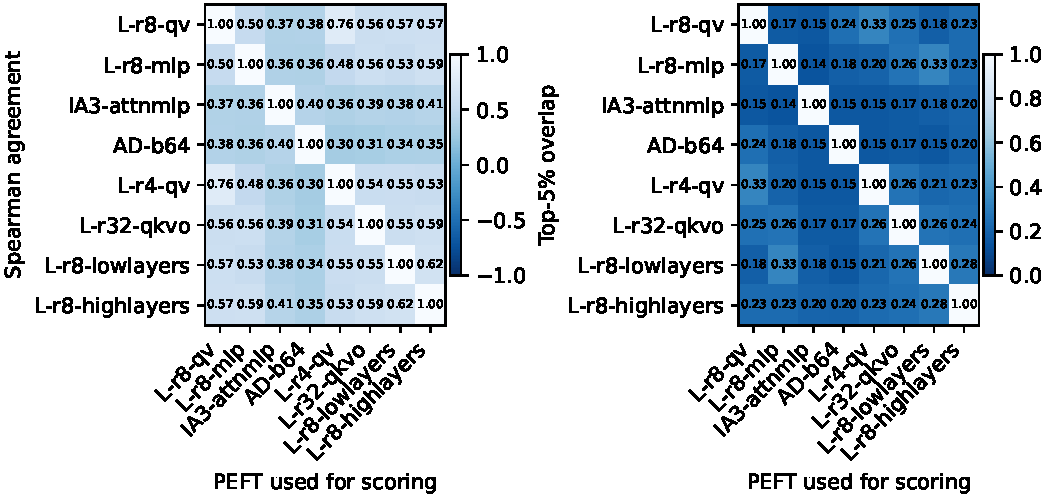
\includegraphics[width=\textwidth]{Figures/fig_motivation_disagreement.pdf}
\caption{Left: Spearman rank agreement between PEFT-conditioned utility rankings. Right: Top-5\% overlap between the corresponding selected examples; lower off-diagonal values indicate stronger configuration dependence.}
\label{fig:motivation-disagreement}
\end{figure*}

The configuration dependence affects downstream performance as well as the rankings. Figure~\ref{fig:motivation-disagreement} shows that independent runs for the same configuration agree more closely than runs across configurations. Changes within one PEFT family preserve more of the ranking, while cross-family changes produce the largest disagreement. Matched selection improves performance by 2.0 points over cross-family reuse and by 1.45 points within LoRA configurations (Supplementary Table~S10 and Figure~S1).

These observations motivate \emph{PEFT-conditioned utility}: the value of training on example $x$ for task $t$ under PEFT configuration $p$. We denote this value by $u(x,p,t)$. A task-only selector omits $p$ and must assign the same ranking to every configuration. Per-PEFT influence selection includes $p$ but recomputes gradients for each target. Our goal is to predict $u(x,p,t)$ while sharing the expensive computations used to learn these scores.

PCU-Select (PEFT-Conditional Utility) enables this sharing through a common representation. It maps every supported configuration to 24 \emph{intervention sites}: selected Transformer module outputs through which PEFT updates affect the backbone. These outputs remain comparable even when PEFT methods train parameter tensors with different shapes. PCU-Select caches sample and task signals at the sites. A structured PEFT code records which sites a configuration affects, its update type, its capacity, and its training recipe. Supplying this code at scoring time preserves configuration information while keeping the cached signals reusable.

A conditional scorer turns the shared signals into a target-specific ranking. Its prediction depends on the candidate example, task sketch, and PEFT code. It learns from two complementary signals: inexpensive labels based on gradient alignment cover the full candidate pool, while short-update labels measure task-sketch loss reductions for a smaller sample. At deployment, the scorer ranks the cached examples for a target configuration and task. PCU-Select then spreads the budget across groups of semantically similar examples to limit near-duplicates. This pipeline moves gradient extraction and label construction offline while retaining a distinct subset for each target.

These design choices amortize target-specific selection across a PEFT registry. We make three contributions:
\begin{itemize}
    \item \textbf{PEFT-conditioned utility.} We define data value as a candidate example's usefulness for a given task and PEFT configuration. We show that both rankings and downstream subset quality change with the target configuration.
    \item \textbf{Intervention-site amortization.} PCU-Select maps different PEFT parameterizations to 24 shared module-output sites. A structured code retains each target's update structure and recipe, enabling configuration-specific rankings without rebuilding gradient datastores; ablations validate both PEFT and task conditioning.
    \item \textbf{Registry-scale quality and cost.} Across four tasks and five seen PEFTs on Llama-2-7B~\cite{touvron2023llama2}, PCU-Select gains 0.74 points over RDS+ and matches per-PEFT LESS within $+0.04$, while cutting four-task PEFT onboarding by $42\times$, from 63.2 to 1.51 GPU-hours.
\end{itemize}

\section{Related Work}

\paragraph{Instruction-data selection.}
Instruction-data selectors usually estimate quality or diversity independently of the target PEFT configuration. LIMA supports instruction tuning with 1,000 curated examples~\cite{zhou2023lima}. Model-based filters instead use judgments or instruction properties: AlpaGasus filters Alpaca examples with LLM judgments~\cite{chen2024alpagasus}, InsTag measures semantic diversity and complexity through instruction tags~\cite{lu2023instag}, and DEITA combines quality, complexity, and diversity~\cite{liu2024deita}. Other methods select for explicit diversity through quality--diversity trade-offs, log-determinant objectives, or partition-aware sampling~\cite{bukharin2023diversity, wang2024diversity, rao2024commonit}. These methods improve data efficiency, but their rankings omit the target PEFT's trainable parameters.

\paragraph{Proxy-model and influence selection.}
Proxy-model selectors provide reusable rankings without computing gradients for every target PEFT. Cherry LLM uses instruction-following difficulty~\cite{li2023cherry}; Superfiltering studies when weak models can rank data for stronger models~\cite{wang2024superfiltering}; and SmallToLarge transfers training-trajectory information from small models to larger targets~\cite{yang2024smalltolarge}. Because these scores encode only example and task information, a PEFT change leaves the ranking unchanged.

Influence-based selectors model training effects more directly, but their gradients tie the score to a target parameterization. Classical influence functions use second-order approximations~\cite{koh2017understanding}, while TracIn accumulates gradient similarities across checkpoints~\cite{pruthi2020tracin}. LESS builds a low-dimensional gradient datastore for instruction selection~\cite{xia2024less}, and DataInf specializes influence approximation for LoRA-tuned generative models~\cite{kwon2023datainf}. Preserving configuration specificity therefore requires rebuilding PEFT-dependent gradients when the target changes. PCU-Select instead conditions one scorer on a structured PEFT code, combining reusable sample signals with a target-specific ranking. Our evaluation compares PCU-Select with both a per-PEFT LESS implementation and an Influence baseline that uses one shared datastore.

\paragraph{Parameter-efficient fine-tuning.}
PEFT methods reduce adaptation cost in different ways, so they expose different trainable parameters. Adapters insert bottleneck modules into Transformer layers~\cite{houlsby2019adapters, pfeiffer2020adapterfusion}, while prefix and prompt tuning optimize continuous prefix states or prompts~\cite{li2021prefixtuning, lester2021prompttuning}. LoRA learns low-rank additive updates~\cite{hu2022lora}, and QLoRA combines quantization with LoRA to reduce memory use~\cite{dettmers2023qlora}. BitFit tunes bias terms~\cite{zaken2022bitfit}, whereas (IA)$^3$ rescales attention and feed-forward activations~\cite{liu2022ia3}. Prior PEFT studies usually compare accuracy, parameter count, memory, or inference overhead while holding the training data fixed. We study the complementary question: whether a fixed candidate pool has the same example ranking across PEFT configurations.

\paragraph{Joint data- and parameter-efficient adaptation.}
The closest methods use PEFT gradients for data selection, but their utility estimates remain specific to one target configuration. DataInf and LESS compute selection signals from LoRA-style training~\cite{kwon2023datainf, xia2024less}. Geometry-aware targeted selection further shows that useful data depends on the directions available to PEFT optimization~\cite{min2026gist}. These methods must regenerate configuration-dependent signals when the target changes.

PCU-Select instead describes each configuration by its intervention sites, update type, capacity, and training recipe. This representation lets one scorer reuse sample and task signals while still producing a different ranking for each configuration.

\section{Problem Formulation}
\label{sec:problem}

We study \emph{cross-PEFT data-efficient fine-tuning}: selecting a small training subset for a target task and PEFT configuration while reusing selection work across configurations. We fix a backbone family and a frozen base model $M_0$. The candidate pool $\mathcal{D}=\{x_i\}_{i=1}^{N}$ contains $N$ instruction--response examples. Each task $t$ provides a \emph{task sketch} $V_t$, a small set from its training or development data. Each PEFT configuration $p\in\mathcal{P}$ specifies a method, trainable locations, capacity, and training recipe. For a selection budget $B$, the ideal subset maximizes held-out task performance:
\begin{equation}
  \mathcal{S}^{*}=\arg\max_{\mathcal{S}\subseteq\mathcal{D},\,|\mathcal{S}|\le B}
  \mathrm{Perf}\!\left(\mathrm{Tune}(M_0,p,\mathcal{S}),V_t^{\mathrm{test}}\right).
  \label{eq:selection-objective}
\end{equation}
Here $\mathrm{Tune}$ adapts $M_0$ with configuration $p$ and subset $\mathcal{S}$, and $\mathrm{Perf}$ evaluates the adapted model. The held-out test set $V_t^{\mathrm{test}}$ defines this ideal objective but never enters training, scoring, or selection; those procedures use only $V_t$. Directly solving Eq.~\eqref{eq:selection-objective} would require training and evaluating many subsets for every target $(p,t)$ pair.

PCU-Select avoids this search by assigning each example a conditional utility: its benefit for task $t$ when training uses configuration $p$. The scorer $s_{\phi}$ approximates this utility for each example:
\begin{equation}
  s_{\phi}(x,p,t)\approx u(x,p,t).
  \label{eq:surrogate}
\end{equation}
The target $u(x,p,t)\in[0,1]$ summarizes task-sketch loss reductions after a few PEFT update steps. PCU-Select rank-normalizes these reductions within groups that share the same PEFT, task, and measurement setting (\S\ref{sec:method}). Including $p$ allows the ranking to change with the trainable subspace; omitting $p$ would force every configuration to share one task-specific ranking. The task sketch $V_t$ identifies the desired task behavior, while $p$ identifies the updates available to the model. Utility is therefore relative to both the task and the PEFT configuration.

\paragraph{Amortization objective.}
A registry changes the cost objective because it serves multiple PEFT configurations and tasks from one candidate pool. Let $P$ be the number of target configurations and $Q$ the number of task sketches. LESS builds one gradient datastore for each configuration and ranks that datastore once for each task. PCU-Select instead pays one shared offline cost, followed by one scoring-and-selection pass for every PEFT--task pair:
\begin{equation}
  \begin{aligned}
  C_{\mathrm{LESS}}(P,Q)
    &=P\!\left(C^{\mathrm{data}}_{\mathrm{LESS}}+
      Q C^{\mathrm{rank}}_{\mathrm{LESS}}\right),\\
  C_{\mathrm{PCU}}(P,Q)
    &=C_{\mathrm{offline}}+PQ C^{\mathrm{pair}}_{\mathrm{PCU}}.
  \end{aligned}
  \label{eq:cost}
\end{equation}
Equation~\eqref{eq:cost} separates four costs. $C^{\mathrm{data}}_{\mathrm{LESS}}$ builds one PEFT-specific datastore, and $C^{\mathrm{rank}}_{\mathrm{LESS}}$ ranks it for one task. $C_{\mathrm{offline}}$ extracts reusable signals and trains PCU-Select once. $C^{\mathrm{pair}}_{\mathrm{PCU}}$ scores and selects data for one target pair. The first expression repeats datastore construction $P$ times, whereas the second pays the offline cost once. Section~\ref{sec:reuse} measures each cost term.

The objective is to retain per-PEFT LESS quality while replacing repeated datastore construction with shared offline work. The supplementary material formalizes the quality criterion and derives the break-even point; Section~\ref{sec:reuse} reports the measured result.

% Equation 4 (the quality criterion) appears in the supplementary material.
\setcounter{equation}{4}

\section{Method: PCU-Select}
\label{sec:method}

PCU-Select learns the conditional utility surrogate in Eq.~\eqref{eq:surrogate} and selects a budgeted subset for a target PEFT--task pair. Figure~\ref{fig:architecture} summarizes two stages. Offline, it extracts reusable sample and task signals, constructs two types of utility label, and trains one scorer. Online, it combines cached sample features with a target $(p^{*},t^{*})$, scores the pool, and distributes budget across semantic clusters. Supplementary Algorithms~S1 and~S2 specify both stages.

\begin{figure*}[t]
\centering
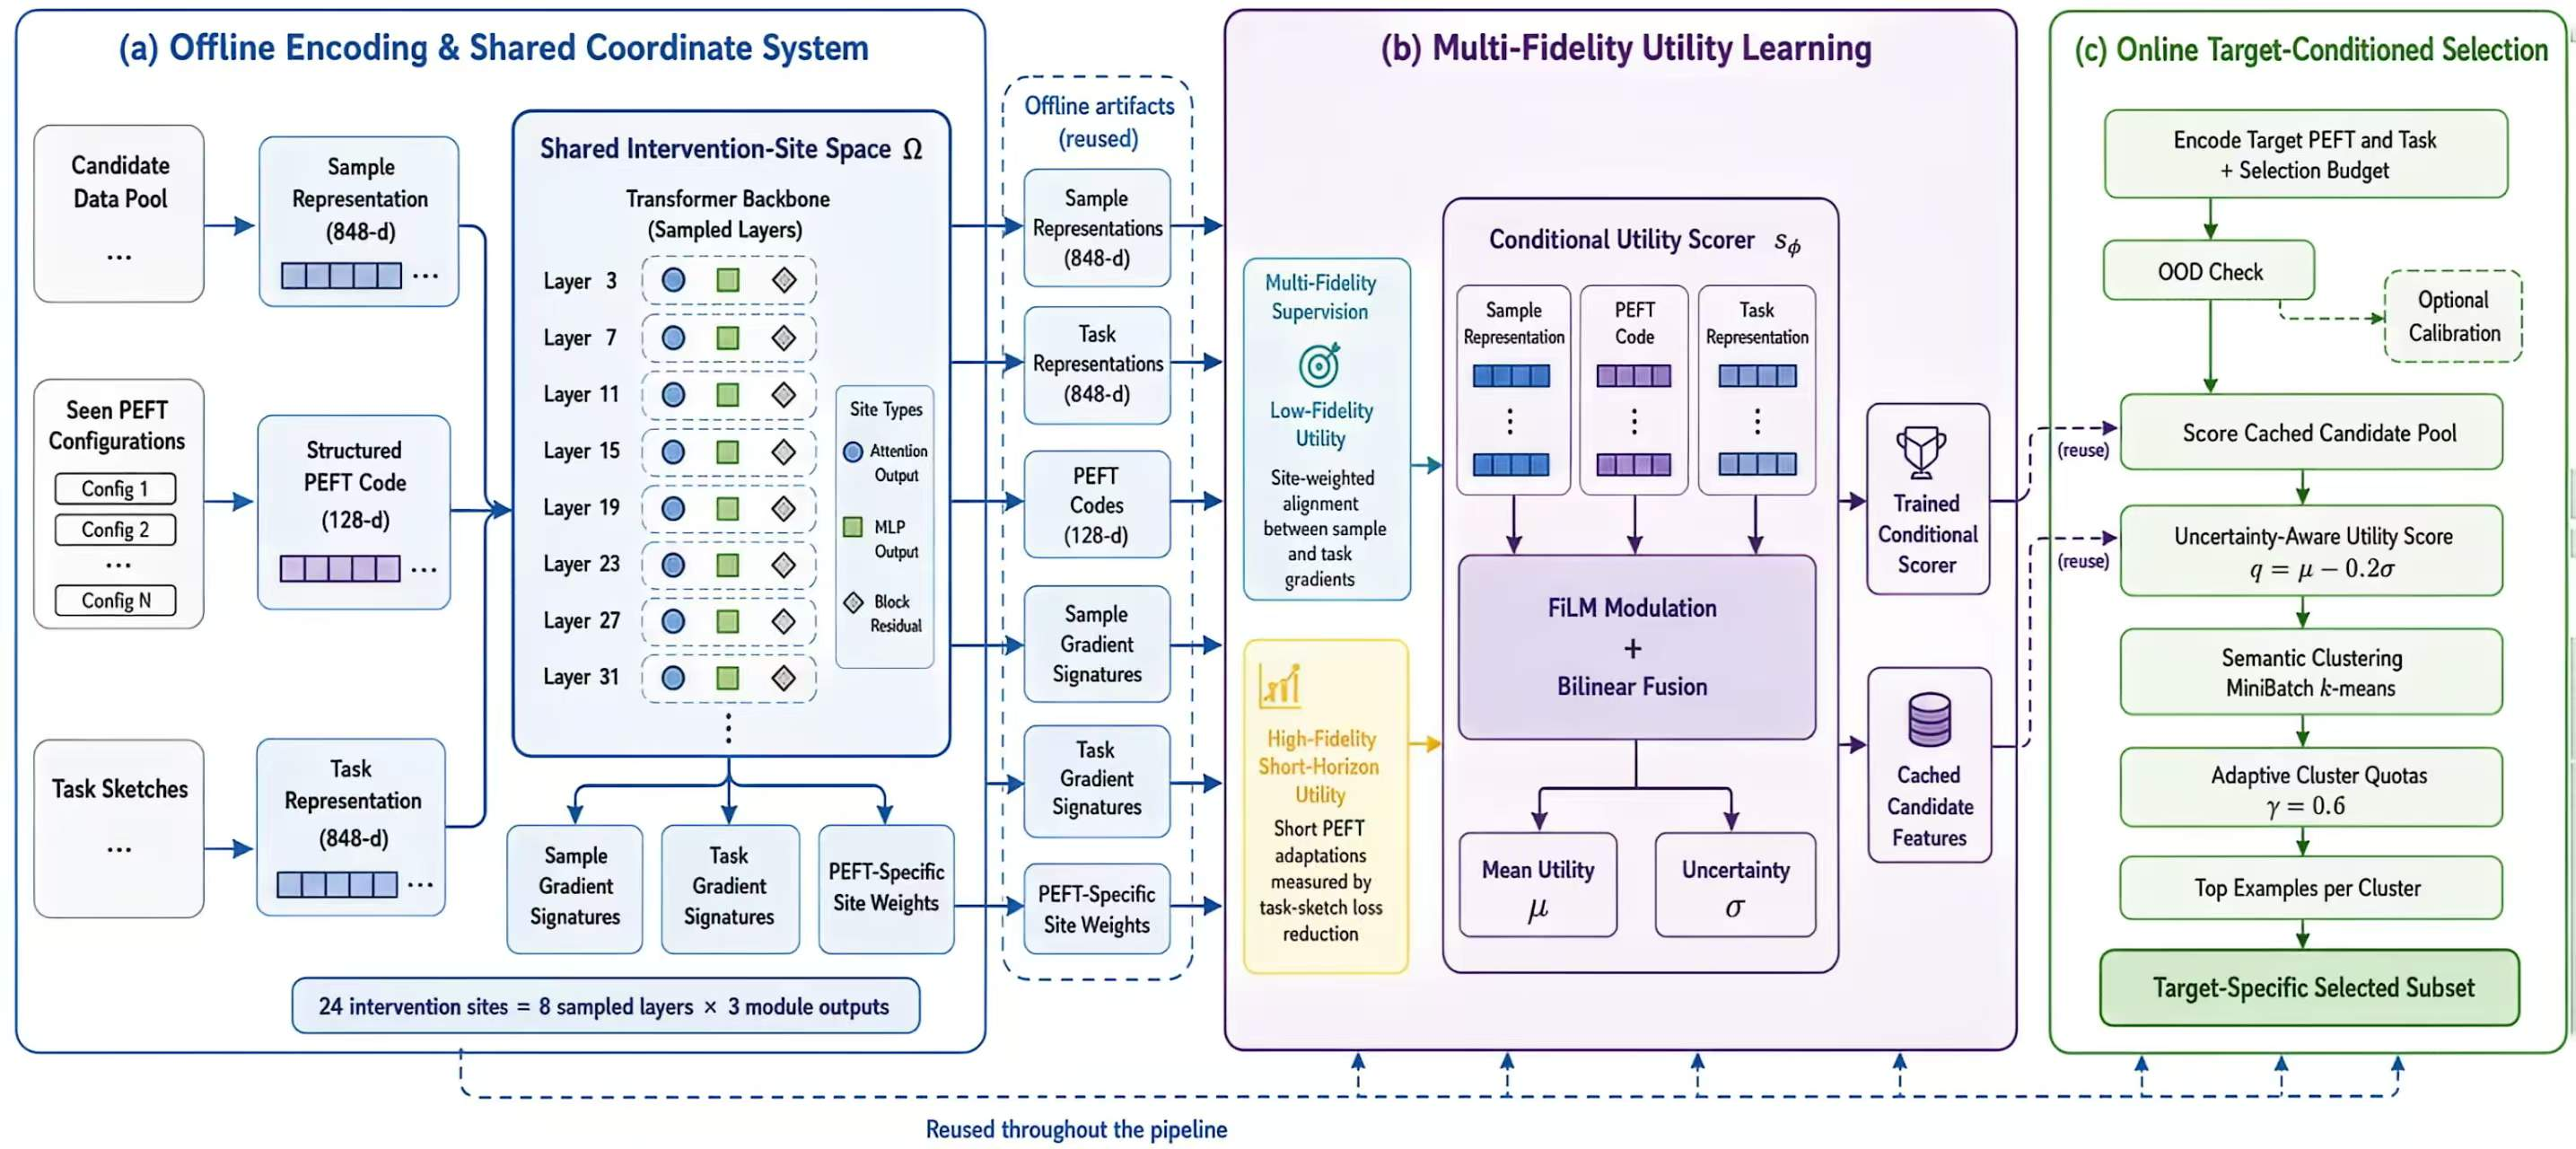
\includegraphics[width=\textwidth]{Figures/image.jpg}
\caption{PCU-Select learns from reusable site-level signals and scores each PEFT--task target online. A 24-site coordinate system aligns sample and task gradients with a 128-dimensional structured PEFT code; proxy and short-update labels provide complementary supervision.}
\label{fig:architecture}
\end{figure*}

\subsection{Shared Intervention Sites Enable Cross-PEFT Reuse}

PEFT families expose parameter tensors with different shapes and roles, so their raw gradients cannot share one cache~\cite{hu2022lora,houlsby2019adapters,liu2022ia3}. PCU-Select instead uses a fixed set $\Omega$ of \emph{intervention sites}. Each site is a selected module output through which a PEFT update affects the backbone. The set $\Omega$ is a shared coordinate system because sample gradients, task gradients, and each PEFT's map of affected sites all use the same index $\omega$.

PCU-Select hooks attention, MLP, and post-residual outputs at eight evenly spaced Transformer layers, giving $|\Omega|=24$. A site's response-loss gradient describes how a sample or task pushes that activation. By the chain rule, PEFT-parameter gradients factor through gradients at the module outputs they modify. Site gradients therefore avoid both full PEFT-parameter reconstruction and shape mismatches between fused and split projections. Post-residual sites place adapters in the same index space as LoRA and (IA)$^3$.

A site index records only \emph{where} a configuration acts. PCU-Select separately encodes operator and capacity features to record \emph{how} it acts and how much it can update. This factorization reuses one sample signature without treating additive, multiplicative, and bottleneck updates as equivalent.

Each configuration maps to a site mask and operator type. Attention LoRA and (IA)$^3$-attention map to attention-output sites. MLP LoRA and (IA)$^3$-FFN map to MLP-output sites, while adapters map to block-residual sites. Prefix tuning maps to attention-output sites. LN Tuning updates Llama-2's per-block RMSNorm scales~\cite{wang2022lntuning,touvron2023llama2}: input-normalization scales map to attention-output sites, and post-attention-normalization scales map to MLP-output sites. The configuration excludes the final model-level RMSNorm. Both site types use the multiplicative operator channel. These mappings define each normalized site weight:
\begin{equation}
  \begin{aligned}
  w_p^{\omega}
  &=\mathrm{mask}(p,\omega)\,\kappa(p,\omega),\\
  \kappa(p,\omega)
  &=\tanh\!\left(\eta\log(1+\mathrm{cap}(p,\omega)/d_{\mathrm{model}})\right),\\
  \tilde{w}_p^{\omega}
  &=w_p^{\omega}/\max(\varepsilon_w,\sum_{\omega'}w_p^{\omega'}).
  \end{aligned}
  \label{eq:site-weight}
\end{equation}
Here $\mathrm{mask}(p,\omega)$ is zero at untouched sites, and $\mathrm{cap}(p,\omega)$ measures trainable capacity. The width $d_{\mathrm{model}}$ normalizes capacity, $\eta$ controls saturation through $\tanh$, and $\varepsilon_w$ keeps the denominator nonzero. Thus, $\tilde{w}_p^{\omega}$ distributes unit weight over the sites used by $p$. Supplementary Table~S8 maps LoRA rank, adapter width, (IA)$^3$ vector count, prefix length, and LN-Tuning scale count to this quantity. Operator type remains separate in $z_p$ because a family-wide scalar would cancel under Eq.~\eqref{eq:site-weight}'s normalization.

\subsection{Shared Representations Preserve Target Specificity}

Shared site indices make signals comparable, but the scorer must still distinguish each sample, task, and PEFT. PCU-Select uses three fixed-length vectors: the sample representation describes the example, the task representation describes the target need, and the PEFT representation describes where and how training acts. Site gradients supply separate label-construction signals.

The sample representation $z_x=[e_x;d_x;a_x]\in\mathbb{R}^{848}$ combines semantic, descriptive, and activation features. The 768-dimensional $e_x$ is the frozen \texttt{sentence-transformers/all-mpnet-base-v2} embedding of the instruction and response~\cite{song2020mpnet,reimers2019sentencebert}. This encoder remains frozen during pool and target-benchmark processing. The 16-dimensional $d_x$ records length, response-LM loss, entropy, and format. The 64-dimensional $a_x$ summarizes response-token hidden states at the eight sampled layers.

Utility is task-relative, so PCU-Select forms $z_t\in\mathbb{R}^{848}$ by mean-pooling $z_x$ over the task sketch's 32 examples. For proxy labels, it separately averages their site gradients into $g_t^{\omega}$. These $24\times256$ values remain outside $z_t$ and serve only label construction.

The PEFT representation records the target trainable subspace. In $z_p=[m_p;c_p;r_p]\in\mathbb{R}^{128}$, the $24\times4$ mask $m_p$ contributes 96 dimensions. Its channels mark active sites, additive updates, multiplicative scaling, and prefix-style control. Two 16-dimensional vectors encode capacity $c_p$ and training recipe $r_p$. At this site resolution, q/v and q/k/v/o LoRA share attention-output sites, while capacity and recipe preserve their projection-level distinction.

Prefix, P-Tuning, and LN Tuning use the same deterministic encoding rules as seen families. The scorer has no learned family lookup or operator centroid. The support policy below decides whether a target uses direct scoring, calibrated scoring, or a per-target selector.

Training these representations requires labels for many $(x,p,t)$ triples, but measuring every PEFT update would defeat amortization. PCU-Select instead uses \emph{multi-fidelity supervision}, which combines labels with different costs and directness. A low-fidelity gradient proxy cheaply covers the pool. High-fidelity short updates directly measure sketch-loss reduction for fewer triples. Together, they learn broad ranking structure and correct errors near the subset cutoff.

The \emph{gradient-proxy label} measures alignment between a sample and the task sketch at sites used by the target PEFT:
\begin{equation}
  u^{\mathrm{lo}}(x,p,t)=\sum_{\omega\in\Omega}\tilde{w}_p^{\omega}
  \cos\!\left(g_x^{\omega},g_t^{\omega}\right).
  \label{eq:ulo}
\end{equation}
Here $g_x^{\omega}$ is the response-token loss gradient at site $\omega$. A Johnson--Lindenstrauss random projection~\cite{johnson1984jl} compresses it to 256 dimensions and unit-normalizes the result. The task-sketch mean gives $g_t^{\omega}$. Equation~\eqref{eq:ulo} therefore measures alignment only at sites used by $p$. All sketches use response-token cross-entropy for these signatures; task-native metrics such as option likelihood, Pass@1, and F1 remain downstream evaluation metrics. Because cosine values can be negative, PCU-Select rank-normalizes them within each $(p,t)$ bucket before proxy distillation and ranking. Cached sample signatures then label many $(x,p,t)$ triples without new gradient extraction.

The \emph{short-update label} measures realized sketch-loss reduction near the subset cutoff. For each sampled triple, PCU-Select uses two anchors $\theta_a$: the base model and a warm checkpoint after adaptation has begun. The horizon $h$ is the number of short-update steps. A mini-batch $\mathcal{B}(x)$ contains the sampled example and seven condition-matched fillers. PCU-Select applies PEFT $p$ for $h$ steps and measures
\begin{equation}
  \Delta(x,p,t,a,h)=L_{V_t}(\theta_a)-
  L_{V_t}\!\left(\mathrm{Adapt}^{h}_{p}(\mathcal{B}(x);\theta_a)\right).
  \label{eq:delta}
\end{equation}
Thus, $\Delta$ is the task-sketch loss before the update minus its loss afterward. Rank-normalized reductions for $h\in\{1,4\}$ from both anchors define $u^{\mathrm{hi}}$. The fillers make this mini-batch effect more stable than a single-example update. PCU-Select allocates 10K short-update labels in three stages. Coverage sampling first spreads labels across the registry without a scorer.

Coverage labels and the proxy then train a provisional scorer. It predicts ranks and a per-triple uncertainty scale, an estimate of prediction noise. Uncertainty sampling selects triples with large scales. Boundary sampling selects large predicted--observed rank disagreements near the cutoff. Every rank normalization compares labels within one PEFT, task, anchor, and horizon bucket.

The proxy cheaply orders the full pool, while short updates target consequential ranking errors. Two anchors test whether utility persists after adaptation begins; two horizons reduce dependence on one update length. Ranking within condition-matched buckets avoids assuming a shared raw-loss scale across tasks or configurations.

\subsection{Conditional Scoring Produces Target-Specific Subsets}

The scorer consumes $(z_x,z_p,z_t)$ and predicts $(\hat{\mu},\hat{\sigma})=s_{\phi}(z_x,z_p,z_t)$. Here $\hat{\mu}$ gives predicted mean utility, while $\hat{\sigma}$ gives a positive, input-dependent uncertainty scale. Separate encoders map the three inputs into hidden vectors. FiLM modulation~\cite{perez2018film} uses the PEFT and task codes to rescale and shift sample features. A bilinear term represents sample--PEFT compatibility.

Stage A distills gradient-proxy ranks to learn broad conditional structure. Stage B continues proxy distillation and adds ranking and regression on short-update labels plus a heteroscedastic uncertainty loss. Here \emph{heteroscedastic} means that predicted noise can differ across triples. PCU-Select selects the Stage B checkpoint on held-out PEFT--task pairs. It also fixes the sketch size, label allocation, anchors, horizons, and scalar selection hyperparameters on these pairs before downstream evaluation.

A target's structural support level determines whether PCU-Select applies the scorer directly or calibrates it. Relative to the seen registry, L0 resembles a seen configuration, L1 makes a larger shift within a seen family, and L2 introduces an unseen family. Seen targets use the trained scorer directly. L0 targets run \emph{zero-shot}: PCU-Select scores a new configuration without target-specific short-update labels. L1 and L2 targets use calibrated scoring when compatible labels exist and a per-target selector otherwise.

After any required calibration, PCU-Select converts the two scorer outputs into a conservative ranking score:
\begin{equation}
  q(x)=\hat{\mu}(x,p^{*},t^{*})-\lambda\hat{\sigma}(x,p^{*},t^{*}),\qquad \lambda=0.2.
  \label{eq:qscore}
\end{equation}
The uncertainty scale reduces the rank of examples whose predicted utility is noisy. It serves as a ranking penalty, not a confidence interval.

Ranking by $q$ alone can over-select near-duplicates, so PCU-Select clusters examples in semantic space before assigning the budget. It allocates budget $B$ across $K$ clusters $C_k$, where $k\in\{1,\ldots,K\}$:
\begin{equation}
  b_k=\mathrm{round}\!\left(
  B\frac{(v_k^{+})^{\gamma}|C_k|^{1-\gamma}}
  {\sum_j(v_j^{+})^{\gamma}|C_j|^{1-\gamma}}\right),\qquad \gamma=0.6.
  \label{eq:quota}
\end{equation}
Here $v_k$ is the mean conservative score among the top 10\% of examples in $C_k$, and $v_k^{+}=\max(v_k,0)$. The factors $v_k^{+}$ and $|C_k|$ balance cluster value and size. For the 300K pool, $K=\max(50,\lfloor\sqrt{N}\rfloor)$ produces 547 clusters of about 548 examples. The reported end-to-end cost is 0.38 GPU-hours per PEFT--task application and includes clustering. PCU-Select takes the top-$b_k$ examples by $q$ within each cluster. Non-positive clusters receive no budget; deterministic remainder handling makes the quotas sum to $B$.

For seen and L0 targets, all gradient extraction and label construction occur offline; online selection uses cached features and scorer forward passes. L1 and calibratable L2 targets add a small label set without rebuilding a target-specific gradient datastore. The evaluation next tests whether this reuse preserves LESS-level quality, reduces registry cost, and transfers across support levels.

\section{Experiments}
\label{sec:experiments}

The evaluation tests whether PCU-Select preserves per-PEFT LESS's average downstream quality, reduces the marginal cost of adding a PEFT, and transfers to new configurations according to their structural support in the training registry. After establishing quality and cost, we examine whether conditioning produces target-specific subsets and identify which components sustain the reusable scorer.

\subsection{Setup}

We evaluate Llama-2-7B~\cite{touvron2023llama2} on GSM8K, HumanEval, MMLU, and TyDiQA~\cite{cobbe2021gsm8k,chen2021humaneval,hendrycks2021mmlu,clark2020tydiqa}, using exact match, Pass@1, accuracy, and F1, respectively. We express these scores as percentages and use their equal-weight macro-average only as a registry-level summary. Per-task results appear in Supplementary Table~S1. From a decontaminated pool of 300K mixed instruction examples, every selector chooses 10\%; the supplementary material gives the reproducibility protocol.

The main comparison covers five configurations seen during scorer training: attention and MLP LoRA, (IA)$^3$, and adapters. The transfer study holds out configurations that vary rank, placement, learning rate, or family. Its unseen-family slice includes Prefix Tuning, P-Tuning, and LN Tuning~\cite{wang2022lntuning}. We instantiate LN Tuning on Llama-2 by updating the scale parameters of both RMSNorm modules in every Transformer block and excluding the final model-level RMSNorm~\cite{touvron2023llama2}. Supplementary Table~S3 lists the full 17-configuration registry.

The four baselines differ in target specificity. \textbf{Random} uses neither task nor PEFT information. \textbf{RDS+}, our representation-similarity baseline, ranks frozen semantic embeddings by similarity to the task-sketch mean but ignores the PEFT configuration. \textbf{Influence}, our shared-datastore gradient baseline, ranks projected base-model gradients from one PEFT-agnostic datastore. \textbf{LESS}, our per-PEFT implementation of gradient-influence selection~\cite{xia2024less}, warms up each target adapter, builds an Adam-preconditioned gradient datastore, and ranks examples by sketch influence. PCU-Select uses its conditional scorer, uncertainty penalty, and adaptive semantic-cluster quotas. The supplementary material gives full specifications.

We hold the backbone, PEFT recipe, training steps, and evaluation protocol constant, so only the selected subset changes. The main table varies target-training seeds 0, 1, and 2 while fixing the selector, scorer, sketch, and pool at seed 0. Matched seeds give every selector the same training randomness. We obtain each descriptive 95\% interval by resampling the evaluated PEFT--task cells under this fixed selection pipeline.

\subsection{PCU-Select Near-Ties Per-PEFT LESS}
\label{sec:quality}

\begin{table*}[t]
\centering
\small
\setlength{\tabcolsep}{4pt}
\begin{tabular}{lrrrrrr}
\toprule
Method & AD-b64 & IA3-attnmlp & L-r16-qkvo & L-r8-mlp & L-r8-qv & Avg. \\
\midrule
Random & 32.79$\pm$0.38 & 31.74$\pm$0.13 & 33.11$\pm$0.23 & 31.97$\pm$0.21 & 31.82$\pm$0.16 & 32.29$\pm$0.16 \\
RDS+ & 35.27$\pm$0.23 & 33.54$\pm$0.26 & 35.00$\pm$0.29 & 34.46$\pm$0.21 & 33.91$\pm$0.17 & 34.44$\pm$0.13 \\
Influence & 35.08$\pm$0.27 & 33.84$\pm$0.26 & 35.24$\pm$0.19 & 34.69$\pm$0.13 & 34.53$\pm$0.22 & 34.68$\pm$0.11 \\
LESS & 35.52$\pm$0.20 & 34.44$\pm$0.13 & 35.80$\pm$0.15 & \textbf{35.13$\pm$0.14} & 34.80$\pm$0.37 & 35.14$\pm$0.14 \\
PCU-Select & \textbf{35.61$\pm$0.40} & \textbf{34.60$\pm$0.21} & \textbf{35.93$\pm$0.30} & 34.56$\pm$0.23 & \textbf{35.18$\pm$0.31} & \textbf{35.18$\pm$0.16} \\
\bottomrule
\end{tabular}
\caption{Each PEFT column reports the equal-weight macro-average of the four task-native percentage scores. Values are mean $\pm$ standard deviation across three matched downstream-training seeds; the selector, task sketch, candidate pool, and scorer are fixed. Across the 20 configuration--task cells, the paired PCU-Select-minus-LESS difference is $+0.04$ points, with a descriptive 95\% interval of $[-0.26,+0.33]$.}
\label{tab:main-results}
\end{table*}


Table~\ref{tab:main-results} shows that PCU-Select improves on the PEFT-agnostic baselines and remains close to target-specific LESS. It gains 0.74 points over RDS+ and wins 17 of 20 PEFT$\times$task cells, with descriptive interval $[+0.38,+1.06]$. It gains 0.50 points over Influence and wins 18 cells, with interval $[+0.21,+0.75]$. Its mean is 0.04 points above LESS, with interval $[-0.26,+0.33]$ and 10 wins in 20 cells.

The LESS comparison varies across tasks. PCU-Select leads on MMLU, has task-level descriptive intervals that cross zero on GSM8K and HumanEval, and trails on TyDiQA and MLP-only LoRA. Task-grouped resampling yields $[-0.15,+0.22]$ for the aggregate gap (Supplementary Table~S1). Together, these results show that PCU-Select improves both PEFT-agnostic baselines and near-ties per-PEFT LESS.

\subsection{Amortization Cuts Four-Task PEFT Onboarding Cost by 42$\times$}
\label{sec:reuse}

\begin{table}[t]
\centering
\small
\setlength{\tabcolsep}{2pt}
\begin{tabular}{lrrrrr}
\toprule
Method & Fixed & Marg. & Total & Quality & Gap \\
\midrule
Random          &  0.0 &  0.0 &   0.0 & 32.29 & $-2.85$ \\
RDS+            &  1.6 &  0.0 &   1.6 & 34.44 & $-0.70$ \\
Influence       & 48.8 &  0.0 &  48.8 & 34.68 & $-0.46$ \\
Reuse-one-LESS  & 63.2 &  0.0 &  63.2 & 34.24 & $-0.90$ \\
\midrule
LESS            &  0.0 & 63.2 & 316.0 & 35.14 & $\phantom{+}0.00$ \\
PCU-Select      & 144.0 & \textbf{1.51} &  151.6 & \textbf{35.18} & $+0.04$ \\
\bottomrule
\end{tabular}
\caption{Quality and selection cost across five seen PEFTs. Costs are GPU-hours
and exclude downstream tuning; \emph{Gap} is the paired difference from
LESS in task-native points. Boldface marks the best quality and marginal cost.}
\label{tab:quality-cost-headline}
\end{table}


Table~\ref{tab:quality-cost-headline} separates \emph{fixed/shared} cost, paid once, from \emph{marginal} cost, paid for each new PEFT. All selector costs exclude the shared 12.8 GPU-hour downstream run. PCU-Select and per-PEFT LESS have near-tied average quality but distribute selection cost differently. LESS has no fixed cost and spends 63.2 GPU-hours per four-task configuration. PCU-Select pays 144.0 GPU-hours once, then 1.51 GPU-hours per new configuration: a $42\times$ lower marginal cost.

The gap comes from configuration reuse. Adding a task to an existing PEFT costs one online-selection pass: 0.38 GPU-hours for PCU-Select and 0.30 for LESS. The PCU-Select value rounds the exact average per-task cost of 0.3775. Adding a PEFT forces LESS to rebuild its datastore, whereas PCU-Select reuses the scorer (Supplementary Table~S5). The cost benefit therefore comes from cross-PEFT reuse.

The fixed-subset shortcut trades away quality. \textbf{Reuse-one-LESS} applies one LESS subset to all five targets; it costs 63.2 GPU-hours but averages 34.24, below RDS+ at 34.44. Reusing a subset selected for one trainable subspace removes the target condition. PCU-Select produces a distinct subset for each target and retains LESS-level average quality.

The measured costs break even at 2.33 four-task configurations; the supplementary material gives the derivation. Serving the five-PEFT registry costs 151.6 GPU-hours with PCU-Select and 316.0 with LESS, a $2.09\times$ reduction.
For targets far from the training registry, optional calibration uses 500 \emph{reduced calibration labels} from one warm anchor and one update step. This procedure costs 1.05 GPU-hours per $(p,t)$, one quarter of the $\approx4.2$ GPU-hours for the full routine. It shifts the worst-case break-even point to 2.50 configurations. For supported four-task configurations that require no calibration, PCU-Select's marginal selection cost is $42\times$ lower than per-PEFT LESS.

\subsection{PEFT Conditioning Produces Target-Specific Subsets}
\label{sec:conditioning}

Selecting for the target LoRA configuration beats reusing another configuration's subset by 1.45 points (21.25 versus 19.79; Supplementary Figure~S1).
Subset differences increase with structural configuration distance, supporting PEFT-conditioned utility; Supplementary Figure~S1 reports the Jaccard and leave-one-configuration-out analyses.

\subsection{Reduced Calibration Narrows the L1 and LN-Tuning Gaps}
\label{sec:transfer}

We next test whether the structural code guides transfer beyond seen targets. Before evaluation, we fix three support levels: L0 resembles a seen configuration, L1 makes a larger shift within a seen family, and L2 introduces an unseen family. Supplementary Table~S3 lists the registry.

\begin{figure}[t]
\centering
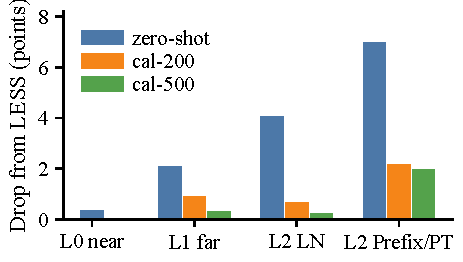
\includegraphics[width=.70\columnwidth]{Figures/fig_ood_calibration.pdf}
\caption{Bars show the three-seed mean of reference minus PCU-Select on GSM8K, HumanEval, and MMLU; Supplementary Table~S11 reports SD. Lower is better; the horizontal axis marks parity. LESS is the reference except for Prefix/P-Tuning (RDS+); L0 is zero-shot only.}
\label{fig:ood-calibration}
\end{figure}

Against LESS, the zero-shot drop grows with structural distance from L0 through L1 to LN Tuning (Figure~\ref{fig:ood-calibration}; Supplementary Table~S11). L0 trails LESS by 0.34 points zero-shot. Adding 500 reduced calibration labels decreases the L1 drop from 2.08 to 0.30 points and the LN-Tuning drop from 4.08 to 0.23. We compare Prefix/P-Tuning with RDS+ because compatible calibration labels are unavailable; their zero-shot score is 6.97 points lower.

The 500-label reduced-calibration setting costs 1.05 GPU-hours per PEFT--task pair, one quarter of the offline routine. Zero-shot covers near-support targets; reduced calibration nearly closes the tested L1 and LN-Tuning mean drops when labels are compatible.

\subsection{Ablations Identify the Useful Components}
\label{sec:ablation}

Removing the PEFT code causes the largest downstream drop, 1.37 points; the task sketch, both label sources, and adaptive semantic coverage also improve quality.
Supplementary Table~S9 reports the full ablation on GSM8K and HumanEval with two representative PEFTs.

\subsection{Limitations}

Our evaluation covers one backbone family, four tasks, and a finite registry; short-update labels approximate contribution after full training. The current method falls back to a per-target selector for Prefix/P-Tuning because compatible calibration labels are unavailable. Its cost advantage begins after 2.33 four-task configurations for direct scoring and 2.50 under the reported worst-case calibration cost, and it applies when the registry requires LESS-level selection quality.

\section{Analysis}
\label{sec:analysis}

\subsection{PEFT Conditioning Produces Target-Specific Subsets}

The reuse experiment showed that a single fixed subset cannot serve a registry; this section shows the converse mechanism---that PCU-Select's one reusable scorer produces a \emph{different} subset for each configuration without recomputing per-target gradients. Appendix Figure~\ref{fig:config-sensitivity} tests whether the PEFT code changes behavior inside the same LoRA family. PCU-Select achieves 21.25 average performance across the configuration scan, compared with 20.70 for LESS, 20.27 for RDS+, and 18.82 for random. The mismatch matrix shows that using the subset selected for the correct target configuration is better than reusing a subset selected for a different configuration by 1.45 points on average. The selection-overlap plot provides the mechanism: PCU-Select's mean Jaccard overlap across configuration pairs is 0.427, while RDS+ remains 0.981 because it is PEFT-agnostic; the overlap broken down by structural axis (rank, placement, module set, family) is in Appendix Table~\ref{tab:overlap}. The Spearman correlation between the ordinal configuration distance and PCU-Select's selection difference is $\rho=0.71$ (95\% CI $[0.52, 0.83]$), confirming that the selection responds to structural distance rather than to noise.

\begin{figure}[H]
\centering
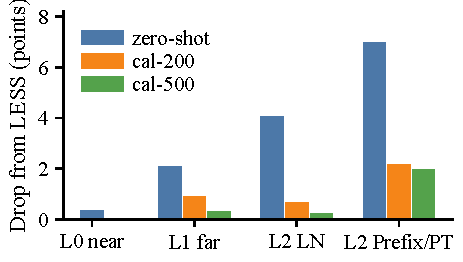
\includegraphics[width=.78\columnwidth]{Figures/fig_ood_calibration.pdf}
\caption{OOD transfer and calibration. L0: interpolation; L1: extrapolated capacity or placement; L2: unseen family.}
\label{fig:ood-calibration}
\end{figure}

\subsection{Ablations Identify the Useful Components}

\begin{table}[!b]
\centering
\small
\setlength{\tabcolsep}{4pt}
\begin{tabular}{lrrr}
\toprule
Variant & Metric & Drop & NDCG \\
\midrule
Full PCU-Select & 19.72$\pm$0.22 & 0.00 & 0.702 \\
No PEFT code & 18.35$\pm$0.41 & 1.37 & 0.526 \\
Family one-hot only & 19.04$\pm$0.29 & 0.68 & 0.602 \\
No task sketch & 18.90$\pm$0.31 & 0.82 & 0.597 \\
No activation signature & 19.24$\pm$0.25 & 0.48 & 0.629 \\
Gradient-proxy labels only & 18.87$\pm$0.34 & 0.85 & 0.563 \\
Short-update labels only & 19.36$\pm$0.27 & 0.36 & 0.639 \\
No uncertainty penalty & 19.44$\pm$0.24 & 0.28 & 0.690 \\
Global top-$k$ & 18.64$\pm$0.38 & 1.08 & 0.684 \\
Uniform clusters & 19.21$\pm$0.28 & 0.51 & 0.709 \\
\bottomrule
\end{tabular}
\caption{Ablations on GSM8K and HumanEval with two representative PEFTs at a 10\% budget (task-native metric averaged over the two tasks, mean$\pm$SD over three seeds). Drop is relative to the full adaptive selector; we measure NDCG against held-out short-update labels.}
\label{tab:ablations}
\end{table}


Table~\ref{tab:ablations} shows that the largest drop comes from removing the PEFT code: performance falls by 1.37 points and, most tellingly, ranking NDCG against held-out utility labels collapses from 0.702 to 0.526---a scale-free signal that the PEFT condition is what lets the scorer order examples correctly. Replacing the structured PEFT code with a family one-hot vector loses 0.68 points, which confirms that rank, placement, capacity, and recipe matter beyond the family name. Removing the task sketch loses 0.82 points, showing that PCU-Select also learns task relativity. Multi-fidelity supervision also matters: low-fidelity-only training loses 0.85 points, while high-fidelity-only training loses 0.36 points because it lacks broad coverage. The adaptive cluster selector beats global top-$k$ by 1.08 points and uniform cluster quotas by 0.51 points. The uniform-cluster variant is instructive: its ranking NDCG ($0.709$) slightly exceeds the full selector's ($0.702$) yet its downstream metric is lower, because equal per-cluster quotas over-sample low-value clusters---ranking quality and subset quality optimize different objectives. The appendix per-task analysis studies the two cells where PCU-Select trails LESS: TyDiQA and MLP-only LoRA.

\subsection{Transfer Protocol for Unseen PEFTs}

The offline scorer serves the seen registry directly, but a deployed system also meets targets outside it, so we turn the OOD analysis into a deployment protocol keyed on a cheap test. A Mahalanobis distance from the seen configuration distribution over $z_p$ assigns each new target to one of three tiers before any labels are drawn: L0 is interpolation (rank/capacity between seen values), L1 is extrapolation (capacity or placement beyond the seen range), and L2 is an unseen PEFT family (Prefix, P-Tuning, BitFit). Because only five seen configurations define the training distribution, the $z_p$ covariance is shrinkage-regularized and the Mahalanobis distance is used coarsely, as a tier assignment rather than a precise density estimate. Zero-shot PCU-Select is within 0.34 points of LESS at L0, trails by 2.08 at L1 (500 calibration labels recover 1.78), and trails by 5.76 at L2 (500 labels recover 5.53); calibration costs 2.1 GPU-hours per target (500 labels through the same $1.89$\,s-per-triple high-fidelity routine used offline), still small relative to a full LESS recomputation. The protocol follows directly (Table~\ref{tab:protocol}): interpolated targets transfer zero-shot, extrapolated targets take a few hundred calibration labels, and unseen families must be calibrated before the scorer is trusted. Calibration is therefore a low-cost repair that keeps far targets inside the amortization regime, not a separate method. Per-level numbers with dispersion and the LESS reference are in Appendix Table~\ref{tab:ood-levels}.

\begin{table}[t]
\centering
\small
\setlength{\tabcolsep}{4pt}
\caption{Deployment protocol from the Mahalanobis tier. Each tier's cost is per target, on top of PCU-Select's amortized 0.18 GPU-hours of online selection; the residual gap to per-PEFT LESS after the recommended action is small (Appendix Table~\ref{tab:ood-levels}).}
\label{tab:protocol}
\begin{tabular}{lll}
\toprule
Tier & Definition ($z_p$ distance) & Recommended action \\
\midrule
L0 & interpolated capacity/placement & zero-shot selection \\
L1 & extrapolated capacity/placement & 200--500 calibration labels \\
L2 & unseen PEFT family & calibrate before trusting \\
\bottomrule
\end{tabular}
\end{table}

\subsection{Limitations}

The current evidence covers one backbone family (Llama-2-7B), four tasks, and a finite PEFT registry, so the claims are cross-PEFT within a single backbone family rather than cross-backbone. PCU-Select also uses short-horizon utility labels rather than full-training marginal contribution as supervision, so the scorer inherits the bias of that proxy; the TyDiQA deficit above is one visible symptom. The candidate pool is decontaminated against all four benchmark test sets using exact, normalized, $13$-gram, and MinHash near-duplicate filters; the appendix reproducibility notes report that this removes $0.58\%$ of the pool. The HumanEval sketch comes from an external code corpus disjoint from the 164 evaluation problems. We cannot fully exclude residual near-duplicate risk below these thresholds. Finally, the cost claim is comparative: PCU-Select amortizes against per-PEFT LESS gradient recomputation, but cheap PEFT-agnostic selectors remain preferable when raw selection cost dominates and a small performance loss is acceptable.

\section{Conclusion}

PCU-Select makes PEFT-conditioned selection reusable, producing target-specific subsets without rebuilding gradient datastores. Across four tasks and five seen configurations, it matches per-PEFT LESS (35.18 versus 35.14), cuts four-task onboarding by $42\times$, and lowers five-PEFT selection cost by $2.09\times$. Calibration recovers 86\% of the L1 gap and 94\% of the LN-Tuning gap; the PEFT-code ablation further supports the role of structural conditioning. Overall, PCU-Select combines target-specific quality, efficient transfer, and low marginal cost in a reusable selector.


% =========================================================
% Ethical Statement
% =========================================================
% Optional. If your paper has ethical considerations, uncomment this block.
% During anonymous submission, make sure it does not reveal author identity.
%
% \section*{Ethical Statement}
% This work studies data selection for parameter-efficient fine-tuning.
% The proposed method is intended to reduce computational cost and improve
% data efficiency. Potential risks include biased data selection if the
% candidate training data or utility supervision contains systematic biases.

% =========================================================
% Acknowledgments
% =========================================================
% Do NOT include acknowledgments in the anonymous submission,
% because funding information, project names, or collaborators may reveal identity.
%
% \section*{Acknowledgments}
% This section should be added only in the camera-ready version.

% =========================================================
% References
% =========================================================
% If you continue using aaai2027.bib, keep this line.
% If you rename your bibliography file to refs.bib, change it to:
% \bibliography{refs}
\bibliography{aaai2027}

% =========================================================
% Technical Appendix
% =========================================================
\clearpage
\appendix

% =========================================================
% Appendix float tuning: pack floats at the top of float-only
% pages instead of vertically justifying them (removes the large
% inter-float gaps), and let more floats share a page with text so
% fewer float-only pages are produced.
% =========================================================
\makeatletter
% Top-align floats on float-only pages; fixed separation; slack at bottom.
\setlength{\@fptop}{0pt}
\setlength{\@fpsep}{10pt plus 0fil}
\setlength{\@fpbot}{0pt plus 1fil}
\setlength{\@dblfptop}{0pt}
\setlength{\@dblfpsep}{10pt plus 0fil}
\setlength{\@dblfpbot}{0pt plus 1fil}
\makeatother
% Allow denser mixing of floats and text.
\renewcommand{\topfraction}{0.9}
\renewcommand{\bottomfraction}{0.8}
\renewcommand{\textfraction}{0.07}
\renewcommand{\floatpagefraction}{0.75}
\renewcommand{\dbltopfraction}{0.9}
\renewcommand{\dblfloatpagefraction}{0.75}
\setcounter{topnumber}{3}
\setcounter{bottomnumber}{2}
\setcounter{totalnumber}{5}
\setcounter{dbltopnumber}{3}

\section{Technical Appendix}
\label{sec:appendix}

\subsection{Quality Criterion and Break-Even Derivation}
\label{sec:appendix-break-even}

The cost comparison applies subject to a user-specified quality tolerance.
Let $\mathrm{Perf}_{\mathrm{PCU}}$ and $\mathrm{Perf}_{\mathrm{LESS}}$ denote
the two selectors' downstream scores. We treat them as tied in quality when
\begin{equation}
  \Delta_{\mathrm{quality}}=\mathrm{Perf}_{\mathrm{PCU}}-\mathrm{Perf}_{\mathrm{LESS}},
  \qquad \lvert\Delta_{\mathrm{quality}}\rvert\le\epsilon.
  \label{eq:quality-tie}
\end{equation}
Here $\epsilon$ is the largest acceptable absolute difference.

Let $P$ and $Q$ denote the numbers of PEFT configurations and tasks,
respectively. PCU-Select is cheaper when its shared offline cost plus its $PQ$
online-selection costs falls below LESS's $P$ datastore-construction costs plus
its $PQ$ ranking costs. Solving this inequality gives
\begin{equation}
  P > P^{\star}=
  \frac{C_{\mathrm{offline}}}
  {C^{\mathrm{data}}_{\mathrm{LESS}}+
  Q(C^{\mathrm{rank}}_{\mathrm{LESS}}-C^{\mathrm{pair}}_{\mathrm{PCU}})},
  \label{eq:break-even}
\end{equation}
provided that the denominator is positive. For $Q=4$, PCU-Select's measured
online cost is 1.51 GPU-hours per configuration, or
$C^{\mathrm{pair}}_{\mathrm{PCU}}=1.51/4=0.3775$ GPU-hours per PEFT--task pair
(displayed as 0.38 in the tables). LESS costs 63.2 GPU-hours per four-task
configuration, while PCU-Select pays 144.0 GPU-hours offline plus 1.51
GPU-hours per configuration. Therefore,
\begin{equation}
  P^{\star}=\frac{144.0}{63.2-1.51}=2.33.
  \label{eq:break-even-measured}
\end{equation}
Because $P$ is integer-valued, PCU-Select costs less at $P\ge3$. If all four
task pairs additionally use 500 reduced calibration labels, the marginal cost
becomes $1.51+4(1.05)=5.71$ GPU-hours and
$P^{\star}=144.0/(63.2-5.71)=2.50$; the integer break-even point remains three
configurations.

\subsection{Per-Task Results Behind the Main Table}
\label{sec:appendix-per-task}

Table~1 in the main paper summarizes four task-native percentage scores: GSM8K
exact match, HumanEval Pass@1, MMLU accuracy, and TyDiQA F1. Because these
metrics have different scales, ceilings, and seed variances, their average can
hide task-level differences. Table~\ref{tab:per-task-compact} therefore reports
them separately. For a baseline $b$, we define
$\Delta b=\mathrm{Perf}_{\mathrm{PCU}}-\mathrm{Perf}_{b}$, so positive values
favor PCU-Select. Each PEFT cell is first averaged over the three
target-training seeds; the task-level value then averages the five seen PEFT
configurations. For LESS, the table also reports a descriptive 95\% interval
obtained by resampling the five paired PEFT-level differences. Parentheses give
the number of configurations for which PCU-Select has the higher seed-averaged
score.

PCU-Select has a higher PEFT-averaged score than RDS+ and Influence on each of
the four tasks. Its comparison with LESS varies by task: the paired
PCU-Select-minus-LESS interval is positive on MMLU ($+0.67$ Acc,
$[+0.24,+1.08]$), crosses zero on GSM8K ($+0.29$ EM,
$[-0.04,+0.58]$) and HumanEval ($-0.04$ Pass@1, $[-0.44,+0.31]$), and is
negative on TyDiQA ($-0.77$ F1, $[-1.18,-0.43]$). These opposing task-level
differences yield the registry-level mean gap of $+0.04$ points reported in the
main paper. The observed registry-average performance is therefore close, but
the task-level results are heterogeneous.

\begin{table*}[t]
\centering
\small
\setlength{\tabcolsep}{5pt}
\begin{tabular}{llrrrr}
\toprule
Task & Metric & PCU & $\Delta$RDS+ & $\Delta$Inf. & $\Delta$LESS (95\% CI) \\
\midrule
GSM8K & EM & 22.20 & +0.55 (5/5) & +0.58 (5/5) & $+0.29$ $[-0.04, +0.58]$ (4/5) \\
HumanEval & Pass@1 & 17.06 & +0.64 (4/5) & +0.24 (4/5) & $-0.04$ $[-0.44, +0.31]$ (2/5) \\
MMLU & Acc & 49.14 & +1.55 (5/5) & +1.00 (5/5) & $+0.67$ $[+0.24, +1.08]$ (4/5) \\
TyDiQA & F1 & 52.30 & +0.22 (3/5) & +0.17 (4/5) & $-0.77$ $[-1.18, -0.43]$ (0/5) \\
\bottomrule
\end{tabular}
\caption{Task-level summary of the main 10\% budget result. Values are averaged over the five seen PEFT configurations. $\Delta$RDS+ and $\Delta$Inf. are absolute native-point gains over PEFT-agnostic baselines; $\Delta$LESS is the paired difference against per-PEFT LESS with a descriptive 95\% cell-resampling interval over PEFT cells. Parentheses report PCU-Select wins among the five PEFT cells for each task; column totals are 17/20, 18/20, and 10/20, respectively.}
\label{tab:per-task-compact}
\end{table*}


\paragraph{Task- and configuration-level differences.}
The largest task-aggregated deficit to LESS occurs on TyDiQA, where PCU-Select
is lower by $0.77$ F1. The largest configuration-aggregated deficit occurs for
MLP-only LoRA (L-r8-mlp), at $0.57$ points. Under this configuration,
PCU-Select's HumanEval and TyDiQA results have downstream-seed SDs of $0.68$
and $0.62$, respectively. These SDs quantify variation across target-training
seeds, not uncertainty predicted by the scorer. The results thus localize the
largest observed discrepancies to TyDiQA and L-r8-mlp, but do not by themselves
identify a causal mechanism.

\subsection{Evaluation Protocols}
\label{sec:appendix-protocols}

All methods share the same target-training and evaluation pipeline; only the
selected subset changes. Target training uses the Llama-2-7B
backbone~\cite{touvron2023llama2}, freezes the backbone, and trains only the
target PEFT. Table~\ref{tab:appendix-peft-registry} lists the per-configuration
learning rates (2e-4 for LoRA, 5e-4 for (IA)$^3$, 3e-4 for adapters, and 1e-4
for L-r64-all). The fixed recipe uses AdamW and a cosine schedule with a $0.03$
warmup ratio. It runs for $1000$ steps with
bfloat16, gradient clipping at $1.0$, and maximum sequence length $1024$. A
per-device batch of $16$ over $8$ GPUs gives a global batch of $128$.

At the 10\% budget, the selected subset holds $30$K examples. The $1000$ steps
therefore process $128$K samples, or about $4.3$ passes over the subset. The
dataloader shuffles the full subset each epoch, so it uses every selected example.
Selected instructions average $\approx512$ tokens, and length-bucketed batches
reduce padding.

With FlashAttention-2~\cite{dao2024flashattention2} and gradient checkpointing,
each step takes approximately $5.8$ wall-clock seconds. At the observed mean
sequence length, this corresponds to about $22$ samples/s in aggregate and
$1.4$K tokens/s per GPU. A 1000-step run takes approximately $96$ minutes, or
$12.8$ GPU-hours under the
$(\text{wall seconds}\times\text{GPU count})/3600$ convention. Because all
selectors use the same target-training recipe and step budget, we exclude
target training from the selection-stage cost comparison.

The primary downstream metric for each task is its standard task-native score,
computed by a task evaluator injected into the training runner. We log
held-out response-LM loss as an auxiliary diagnostic (\texttt{eval\_loss}) but use
only the primary task metric for comparison. Concrete per-task decoding and
scoring protocols are:

\begin{itemize}
  \item \textbf{GSM8K (exact match).} Chain-of-thought generation~\cite{cobbe2021gsm8k} with greedy
    decoding; the evaluator extracts the final numeric answer and checks exact
    match.
  \item \textbf{HumanEval (Pass@1).} The standard unbiased Pass@1 estimator~\cite{chen2021humaneval}:
    sampling at temperature $0.2$ with $n{=}20$ samples per problem, scored by
    unit-test execution. This is a multi-sample estimate of Pass@1, not a single
    greedy sample.
  \item \textbf{MMLU (accuracy).} Log-likelihood scoring~\cite{hendrycks2021mmlu} of the four answer
    options; the evaluator selects the highest-likelihood option without
    free-form generation.
  \item \textbf{TyDiQA-GoldP (F1).} Greedy decoding of the answer span~\cite{clark2020tydiqa}, scored
    with token-level F1 against the gold answers.
\end{itemize}

An evaluation adapter supplies these task-specific evaluators to the runner
through the \texttt{-{}-task-metric-factory} hook. We use the same fixed decoding
and scoring settings for every selector; they define the metrics in this study
and need not match every public evaluation harness.

Under our evaluation pipeline, untuned Llama-2-7B~\cite{touvron2023llama2}
scores $13.9$ on GSM8K, $12.4$ on HumanEval, $43.9$ on MMLU, and $46.2$ on
TyDiQA. Our MMLU value is not directly comparable with Meta's reported $45.3$
because the prompt and evaluation harness differ. Every selector-trained model,
including Random, exceeds the corresponding untuned score on all four tasks.
Random therefore serves as the reference for gains beyond uniform subset
selection.

\subsection{Reproducibility Supplement}
\label{sec:appendix-repro}

This section records the implementation details needed to reproduce the
reported experiments. It pins the public releases and states the
experiment-specific conversion, sampling, and evaluation rules explicitly.

\paragraph{Data provenance and deduplication.}
The candidate pool holds 300K mixed instruction examples drawn from seven public
instruction corpora. Table~\ref{tab:appendix-provenance} identifies the public
snapshot, split, record conversion, and final contribution of every source.

\begin{table*}[t]
\centering
\small
\setlength{\tabcolsep}{3pt}
\begin{tabular}{@{}>{\raggedright\arraybackslash}p{.17\textwidth}
                    >{\raggedright\arraybackslash}p{.29\textwidth}
                    >{\raggedright\arraybackslash}p{.38\textwidth}r@{}}
\toprule
Source & Public release used & Conversion to an instruction--response record & Final rows \\
\midrule
FLAN v2~\cite{longpre2023flan} & \texttt{Open-Orca/FLAN}, third-party FLAN 2022
  materialization, rev.\ \texttt{6845b1b3}, train partitions & Published
  \texttt{inputs} $\rightarrow$ instruction and \texttt{targets}
  $\rightarrow$ response; stratify by component task & 110{,}000 \\
OpenOrca~\cite{lian2023openorca} & \texttt{Open-Orca/OpenOrca}, default/train,
  rev.\ \texttt{aaeb6859} & Concatenate nonempty \texttt{system\_prompt} and
  \texttt{question}; use \texttt{response} as the target; stratify across the
  released GPT-4 and GPT-3.5 partitions & 70{,}000 \\
Tulu v2 SFT mix~\cite{ivison2023camels} &
  \texttt{allenai/}\allowbreak\texttt{tulu-v2-sft-mixture}, default/train,
  rev.\ \texttt{0bc269ee} & Retain alternating user/assistant messages and
  serialize the preceding turns as the instruction; stratify by the released
  \texttt{dataset} field & 50{,}000 \\
OASST1~\cite{kopf2023openassistant} & \texttt{OpenAssistant/oasst1},
  2023-04-12 release, default/train, rev.\ \texttt{fdf72ae0} & Reconstruct
  English conversation trees and pair each prompter turn with its highest-ranked
  positively reviewed assistant child & 30{,}000 \\
CodeAlpaca 20K~\cite{chaudhary2023codealpaca} &
  \texttt{sahil2801/CodeAlpaca-20k}, rev.\ \texttt{152bb5e9}, all 20{,}022
  source rows & Concatenate \texttt{instruction} and nonempty \texttt{input};
  use \texttt{output} as the response & 20{,}000 \\
Dolly 15K~\cite{conover2023dolly} &
  \texttt{databricks/}\allowbreak\texttt{databricks-dolly-15k} v1.0, train,
  rev.\ \texttt{bdd27f4d} & Concatenate \texttt{instruction} and nonempty
  \texttt{context}; use \texttt{response} as the target & 15{,}000 \\
WizardLM Evol-Instruct 70K~\cite{xu2024wizardlm} &
  \texttt{WizardLMTeam/}\allowbreak\texttt{WizardLM\_evol\_}%
  \allowbreak\texttt{instruct\_70k}, train,
  rev.\ \texttt{16b48bd8} & Use \texttt{instruction} as the prompt and
  \texttt{output} as the response & 5{,}000 \\
\midrule
Total & & & 300{,}000 \\
\bottomrule
\end{tabular}
\caption{Candidate-pool provenance, pinned public releases, and record
construction. Revision strings are eight-character prefixes of the public
repository commits. Counts are final post-filter contributions.}
\label{tab:appendix-provenance}
\end{table*}

We apply one sampling rule to all seven releases. Within each source, a PCG64
generator with seed 0 shuffles source-native IDs (or original row indices when
no ID is provided). We scan this order until the source reaches its target
quota. FLAN v2, Tulu v2, and OpenOrca preserve the proportions of their eligible
rows across FLAN component tasks, Tulu's \texttt{dataset} field, and OpenOrca's
GPT-4/GPT-3.5 partitions, respectively. Largest-remainder rounding converts
these proportions to integer stratum quotas. Rejected or duplicate records are
replaced by later records from the same source and stratum, so both source and
stratum totals remain fixed. We preserve the upstream source ID with every
retained record.

Deduplication then runs in three stages. First, it removes exact duplicates by
the content hash of the normalized instruction--response pair. Second, it
removes normalized-string matches after lowercasing and stripping whitespace and
punctuation. Third, MinHash LSH removes near-duplicates using 128 permutations
and a Jaccard threshold of $0.8$. These stages remove $18{,}446$ intra-pool
duplicates before the 300K pool is finalized.

Licensing follows the pinned public releases. The OpenOrca and WizardLM dataset
cards record MIT, although upstream terms may also apply. OASST1 uses
Apache-2.0, CodeAlpaca uses CC-BY-NC-4.0, and Dolly uses CC-BY-SA-3.0. FLAN
components retain their component-specific licenses. The Tulu v2 wrapper is
distributed under ODC-BY-1.0, while its constituent sources retain their own
terms. We use all non-commercial or mixed-license components only for
non-commercial research.

\paragraph{Benchmark decontamination.}
We decontaminate the pool against the test items of GSM8K, HumanEval, MMLU, and
TyDiQA. The filter checks exact matches, normalized-string matches, $13$-gram
overlap, and MinHash LSH near-duplicates. The $13$-gram stage removes candidates
with Jaccard overlap of at least $0.5$; the MinHash stage uses a threshold of
$0.8$. The filter removes $1{,}742$ pre-finalization candidates ($0.58\%$ of the
pool size). We then backfill from the same source buckets to keep the final pool
at 300K examples, so Table~\ref{tab:appendix-provenance} reports final
post-filter counts. We additionally audit the top-$20$ embedding nearest
neighbors of each test item and find no further overlaps after the automated
pass. All reported results are on the decontaminated pool.

\paragraph{Task sketch construction and HumanEval.}
Each task sketch contains 32 examples drawn with fixed seed 0 and stratified by
response length. For GSM8K, MMLU, and TyDiQA, we sort the eligible training or
development records by response character count, split them into three equal
index ranges, and use Python's \texttt{random.Random(0)} to draw 11, 11, and 10
examples from the short, medium, and long ranges. Every sketch remains disjoint
from its task's evaluation split.

HumanEval has no official training or development split. Its sketch is therefore
source-balanced: 16 examples come from the \texttt{full}/\texttt{train} split
(374 rows) of MBPP~\cite{austin2021program}, public revision
\texttt{4bb6404f}, and 16 come from the CodeAlpaca 20K release pinned in
Table~\ref{tab:appendix-provenance}. For MBPP, \texttt{text} is the instruction
and the canonical \texttt{code} solution is the response; the tests are retained
for decontamination and auditing but are not appended to either field. Within
each source, we filter against the 164 HumanEval evaluation problems, form
response-character-length terciles, and use \texttt{random.Random(0)} to draw 6,
5, and 5 examples from the short, medium, and long terciles, respectively. Exact
content matching and AST-normalized function-signature matching are applied
before sampling.

Because the candidate pool also contains CodeAlpaca, we test all 32 sketch items
against the pool and exclude every content-hash or AST-signature match before
selection; the CodeAlpaca quota is then refilled from its seeded order. Thus the
sketch is disjoint from both the HumanEval evaluation set and the candidate
pool. We enforce the same disjointness for every selector because the sketch is
the shared selection signal.

\paragraph{PEFT registry.}
Table~\ref{tab:appendix-peft-registry} lists all 17 PEFT configurations:
five seen, nine unseen same-family configurations, and three unseen families.
The unseen-configuration transfer study evaluates eight held-out
targets---L-r32-qkvo, AD-b16, L-r64-all, AD-b256, L-r8-highlayers, PRE-l16,
PT-l32, and LN---while the configuration-sensitivity study uses the additional
LoRA variants. All use $1000$ steps, a cosine schedule, and $0.03$ warmup;
learning rates vary by configuration.
The LN configuration trains the \texttt{input\_layernorm} and
\texttt{post\_attention\_layernorm} scale parameters in every Transformer
block and excludes the final model-level RMSNorm.

\begin{table*}[t]
\centering
\small
\setlength{\tabcolsep}{4pt}
\begin{tabular}{@{}llllccl@{}}
\toprule
Config & Family & Target modules & Capacity & LoRA scaling & LR & Group \\
\midrule
L-r8-qv        & LoRA      & q, v                       & $r{=}8$   & 16  & 2e-4 & seen \\
L-r16-qkvo     & LoRA      & q, k, v, o                 & $r{=}16$  & 32  & 2e-4 & seen \\
L-r8-mlp       & LoRA      & up, down                   & $r{=}8$   & 16  & 2e-4 & seen \\
IA3-attnmlp    & IA$^3$    & k, v, down                 & --        & --  & 5e-4 & seen \\
AD-b64         & Adapter   & block-residual             & $b{=}64$  & --  & 3e-4 & seen \\
\midrule
L-r4-qv        & LoRA      & q, v                       & $r{=}4$   & 8   & 2e-4 & unseen-config \\
L-r32-qkvo     & LoRA      & q, k, v, o                 & $r{=}32$  & 64  & 2e-4 & unseen-config \\
L-r64-all      & LoRA      & q, k, v, o, up, down, gate & $r{=}64$  & 128 & 1e-4 & unseen-config \\
L-r8-lowlayers & LoRA      & q, v (low third)           & $r{=}8$   & 16  & 2e-4 & unseen-config \\
L-r8-highlayers& LoRA      & q, v (high third)          & $r{=}8$   & 16  & 2e-4 & unseen-config \\
L-r16-hlr      & LoRA      & q, k, v, o                 & $r{=}16$  & 32  & 5e-4 & unseen-config \\
AD-b16         & Adapter   & block-residual             & $b{=}16$  & --  & 3e-4 & unseen-config \\
AD-b256        & Adapter   & block-residual             & $b{=}256$ & --  & 3e-4 & unseen-config \\
IA3-attnonly   & IA$^3$    & k, v                       & --        & --  & 5e-4 & unseen-config \\
\midrule
PRE-l16        & Prefix    & attention                  & len${=}16$& --  & 2e-4 & ood-family \\
PT-l32         & P-Tuning  & attention                  & len${=}32$& --  & 2e-4 & ood-family \\
LN             & LN Tuning & input/post-attn RMSNorm    & 2 scales/layer & -- & 2e-4 & ood-family \\
\bottomrule
\end{tabular}
\caption{Full PEFT registry (all 17 configurations). ``LoRA scaling'' is the
LoRA $\alpha$ hyperparameter and is distinct from the intervention-site weight
$\tilde{w}_p^\omega$ defined in the main paper; it applies only to LoRA rows.
Adapters are single post-block residual bottlenecks (one per layer); IA$^3$
scales the listed activations. LN Tuning updates per-block RMSNorm scales~\cite{wang2022lntuning,touvron2023llama2}.
Learning rates for the three OOD-family targets
use the registry default (2e-4). Layer placement is all layers unless noted;
low/high-third placements use the bottom/top $\lceil n/3 \rceil$ layers of the
32-layer backbone.}
\label{tab:appendix-peft-registry}
\end{table*}

\paragraph{Intervention sites and gradient signatures.}
The site space $\Omega$ provides a shared coordinate system across PEFT families.
It contains $24$ sites: $8$ layers $\times\ 3$ module outputs per layer
(\texttt{attn\_out}, \texttt{mlp\_out}, and \texttt{block\_residual}). Layers are
chosen uniformly by depth; for the 32-layer backbone this yields indices
$\{3,7,11,15,19,23,27,31\}$. Each site carries a Johnson--Lindenstrauss random
projection~\cite{johnson1984jl} $\Phi_\omega \in \mathbb{R}^{256 \times 4096}$ with entries drawn
$\mathcal{N}(0, 1/256)$ under a per-site seed
$\mathrm{SHA256}(\texttt{site}, \texttt{global\_seed}{=}0)$; projected gradients
are $L_2$-normalized per row. Each sample's signature contains $24\times256$
values. In bfloat16, these projected gradients occupy approximately $3.69$~GB
($3.43$~GiB) for the 300K-example pool. They are stored as a memory-mapped array
and reused during offline proxy-label construction; online PCU-Select scoring
uses cached $z_x$ features rather than this gradient store. A configuration
activates sites through its mask and the capacity factor
$\kappa(p,\omega)=\tanh\!\big(\eta\log(1+\mathrm{cap}(p,\omega)/d_{\mathrm{model}})\big)$,
with $\eta{=}1.0$. Operator type enters the explicit PEFT code rather than a
scalar site prior; Table~\ref{tab:capacity} gives the family-specific capacity
mapping.

\paragraph{Conditional scorer.}
The conditional scorer estimates a sample's utility for a specific task and
PEFT configuration. It has three input towers: sample
$z_x \in \mathbb{R}^{848}$, PEFT condition $z_p \in \mathbb{R}^{128}$, and task
sketch $z_t \in \mathbb{R}^{848}$.
Each tower uses a LayerNorm--Linear--GELU--Linear--LayerNorm MLP. Let
$h_x,h_t\in\mathbb{R}^{256}$ and $h_p\in\mathbb{R}^{128}$ denote the three tower
outputs. The concatenated condition $[h_p;h_t]$ produces 256-dimensional FiLM
scale and shift vectors~\cite{perez2018film}, which modulate $h_x$. In parallel,
a bilinear layer maps $(h_x,h_p)$ to a 64-dimensional interaction vector. The
concatenated 320-dimensional representation passes through a
Linear--GELU head that maps it to 256 dimensions. Two linear output heads then
predict mean utility $\widehat{\mu}_{\phi}$ and an example-dependent uncertainty
scale $\widehat{\sigma}_{\phi}$; the latter uses softplus with a floor of
$10^{-3}$.

We use $\widehat{\sigma}_{\phi}$ as a ranking penalty.
On held-out labels, its predicted standard deviation tracks realized error with
a 10-bin expected calibration error of $0.043$. In the downstream ablation,
setting the uncertainty penalty to zero lowers the reported average by $0.28$
points (Table~\ref{tab:ablations}).

Training separates cheap proxy learning from expensive short-update supervision.
Phase A pretrains on the gradient proxy for $3$ epochs at lr $3\times10^{-4}$
with loss weights (rank, reg, proxy, unc) $=(0,0,1,0)$. Phase B jointly fine-tunes
for $2$ epochs at lr $10^{-4}$ with weights $(1.0, 0.3, 0.5, 0.2)$. Both phases
use AdamW, batch size $256$, and gradient clipping at $1.0$. The four losses are a
BPR-style pairwise ranking loss, a Huber regression loss against short-update
labels, a Huber proxy-distillation loss against the gradient-proxy labels, and a
Gaussian negative-log-likelihood uncertainty loss. We track ranking NDCG on a
held-out split of PEFT/task pairs that excludes two configurations and one task
from Phase B. We keep the Phase-B checkpoint with the best held-out NDCG. The
scorer uses no dropout.

\paragraph{Selection, clustering, and quotas.}
At application time, the scorer ranks each example by
$q = \mu - \lambda\,\sigma$ with uncertainty penalty $\lambda{=}0.2$. The
penalty favors examples with high predicted utility and lower uncertainty.
Ranking alone can concentrate the subset in a few semantic regions, so PCU-Select
adds cluster-level coverage. It applies MiniBatch
$k$-means~\cite{sculley2010minibatch} to the joint
embeddings. It uses $k = \max(50, \lfloor\sqrt{N}\rfloor)$, batch size $4096$,
$n_{\text{init}}{=}3$, and random state $0$. Adaptive quotas allocate budget $B$
across clusters by
$b_k = \mathrm{round}\!\big(B\, (v_k^+)^{\gamma}\, |C_k|^{1-\gamma} / Z\big)$ with
$\gamma{=}0.6$. Here $v_k$ is the mean conservative score $q$ among the top
10\% of examples in cluster $C_k$, $v_k^+=\max(v_k,0)$, and
$Z=\sum_j(v_j^+)^\gamma |C_j|^{1-\gamma}$. The algorithm distributes
remainders by descending weight and trims over-allocation from the
lowest-weight clusters.

Targets far from the seen registry can additionally calibrate the scorer with a
small label set. The calibrated mean is
$\widehat{\mu}_{\mathrm{cal}}=\widehat{\mu}_{\phi}
+W_{\mathrm{cal}}[z_x;z_p;z_t]+b_{\mathrm{cal}}$. We freeze the shared scorer
and fit only the zero-initialized residual parameters $W_{\mathrm{cal}}$ and
$b_{\mathrm{cal}}$ for 200 epochs at lr $5\times10^{-3}$ (Adam, MSE). These
deployment calibration labels $u^{\mathrm{hi}}_{\mathrm{cal}}$ are a reduced form of the
offline short-update labels $u^{\mathrm{hi}}$. They use only the warm anchor and
horizon $h{=}1$, rather than both anchors and both horizons. Each label therefore
costs one quarter of the full offline routine in
Eq.~\eqref{eq:uhi-offline}. An offline label costs
$84.0/10{,}000=0.0084$ GPU-hours, while a calibration label costs
$\approx0.0021$ GPU-hours. Budgets of 200 and 500 labels therefore cost $0.42$
and $1.05$ GPU-hours per PEFT--task pair. The full routine would cost about four
times more. We use $200$ or $500$
$u^{\mathrm{hi}}_{\mathrm{cal}}$ labels for the OOD study.

\paragraph{Structural support levels.}
The structural support levels determine whether a PEFT code that differs from
the training registry is evaluated zero-shot or with calibration. The reported
$z_p\in\mathbb{R}^{128}$ contains only the site/operator mask, capacity, and
recipe vectors. Prefix, P-Tuning, and LN Tuning use the same
deterministic encoding rules as the seen families; no centroid, learned family
lookup, or functional fingerprint enters the reported model. We fixed this
registry-relative taxonomy before evaluating the held-out targets. \textbf{L0}
contains near-support
same-family targets (L-r32-qkvo and AD-b16). \textbf{L1} contains farther
same-family shifts (L-r64-all, AD-b256, and L-r8-highlayers). \textbf{L2}
contains unseen families (PRE-l16, PT-l32, and LN). These levels define
registry-relative structural support. L1 and L2 targets use the reduced
calibration protocol described above; their results test whether a small
target-specific label set can repair a larger structural shift.

\begin{table}[t]
\centering
\small
\setlength{\tabcolsep}{3pt}
\begin{tabular}{@{}p{.18\columnwidth}p{.29\columnwidth}p{.45\columnwidth}@{}}
\toprule
Level & Definition & Evaluation mode \\
\midrule
L0 & near-support & zero-shot selection \\
L1 & far-support & 200--500 labels (0.42--1.05 GPU-h) \\
L2-LN & unseen family; labels available & 200--500-label calibration \\
L2-Prompt & Prefix/P-Tuning & 200--500-label calibration \\
\bottomrule
\end{tabular}
\caption{Transfer-evaluation protocol for each registry-defined support level.
Costs are per PEFT--task pair, in addition to 0.38 GPU-hours for online
selection.}
\label{tab:protocol}
\end{table}

\paragraph{Gradient-proxy and short-update labels.}
Short-update supervision concentrates expensive labels where they provide
different kinds of information. It samples $10{,}000$ triples using a
$0.5/0.3/0.2$ split. Coverage sampling spans clusters, PEFT families, capacity
buckets, and tasks. Uncertainty sampling prioritizes large
$\widehat{\sigma}_{\phi}\,(1+0.5\,\mathrm{ReLU}(\hat{u}_{\text{lo}}))$, while boundary
sampling targets disagreement between predicted and observed ranks. Each label
measures a short-update loss reduction on the sketch from two frozen anchors---$\theta_{\text{base}}$
(the pretrained backbone) and $\theta_{\text{warm}}$ (a rank-8 attention-only LoRA
trained for $200$ steps at lr $10^{-4}$). Each short update
$\mathrm{Adapt}^{h}_{p}$ uses one sampled example and $7$ in-bucket fillers.
The fillers stabilize the update relative to a single-example step. The
final label aggregates the rank-normalized reductions across horizons and anchors:
\begin{equation}
\label{eq:uhi-offline}
  u^{\mathrm{hi}}=\tfrac{1}{|A|}\sum_{a\in A}\sum_{h\in\{1,4\}} w_h\,
  \widetilde{\Delta}_{a,h}.
\end{equation}
It uses weights $w_1{=}0.4,\ w_4{=}0.6$ and anchors
$A=\{\text{base},\text{warm}\}$. The term $\widetilde{\Delta}_{a,h}$ is the
reduction defined by the main paper's short-update equation, rank-normalized within its PEFT, task,
anchor, and horizon bucket.

\paragraph{Cost model and seeds.}
We measure all costs on $8{\times}$NVIDIA H20-96GB (SXM, bfloat16, NVLink)
as $(\text{wall seconds} \times \text{GPU count}) / 3600$. PCU-Select pays
144.0 GPU-hours once: 48.0 for feature extraction, 4.8 for gradient-proxy
labels, 84.0 for short-update labels, and 7.2 for scorer training. Dividing the
1.51 GPU-hour four-task measurement by four gives an exact average per-task cost
of 0.3775 GPU-hours, displayed as 0.38. LESS costs
62.0 per PEFT datastore plus 0.30 per task ranking, hence 63.2 for four tasks.
Onboarding a new four-task PEFT therefore costs 1.51 GPU-hours for PCU-Select
versus 63.2 for LESS, a $42\times$ marginal-cost reduction. The shared 12.8
GPU-hour downstream cost applies to each PEFT--task--seed run, so the selection
comparison excludes it. For four tasks, break-even is
$P^\star=144.0/[62.0+4(0.30-0.3775)]=2.33$ configurations.
The pipeline fixes selector-scorer training, task-sketch sampling, and pool
ordering at seed 0. Reported SDs vary target-training seeds ($0,1,2$) with the
selector and scorer pipeline fixed. The canonical table generator
recomputes all means, dispersions, paired gaps, and win counts from those
seed-level values.

Two supplementary tables bound the cost claim. Table~\ref{tab:hf-budget} varies
the offline short-update label budget. The 10K default is the smallest evaluated
budget that preserves the aggregate quality tie. Smaller budgets reduce offline
cost and the break-even point but also reduce quality, making the offline
investment a tunable trade-off. Table~\ref{tab:pool-scaling} separates the online
timing components. At 300K, the instrumented scorer and clustering timers sum to
0.360 GPU-hours. The end-to-end measurement is 0.3775, leaving 0.0175 GPU-hours
of uninstrumented overhead, which we retain explicitly rather than assigning to
either component. Under a linear datastore-cost extrapolation anchored at
LESS's measured 300K cost, PCU-Select's end-to-end online cost is approximately
$170\times$ smaller across the reported pool sizes.

\begin{table}[t]
\centering
\small
\setlength{\tabcolsep}{6pt}
\begin{tabular}{lrr}
\toprule
New registry entry & PCU-Select & LESS \\
\midrule
One new task, existing PEFT   & 0.38 & 0.30 \\
One new PEFT, four tasks       & 1.51 & 63.2 \\
\bottomrule
\end{tabular}
\caption{The amortization advantage is cross-PEFT, not cross-task. Adding a task
to an existing PEFT costs each selector one online-selection pass; adding a PEFT for
four tasks forces LESS to rebuild its datastore while PCU-Select reuses the
offline scorer. Selection-stage GPU-hours; PCU-Select's per-task entry rounds
the exact average $1.51/4=0.3775$.}
\label{tab:cost-axes}
\end{table}

\begin{table}[t]
\centering
\small
\setlength{\tabcolsep}{5pt}
\caption{Offline high-fidelity label budget sets the quality--break-even
trade-off. High-fidelity labeling is $58\%$ of offline cost, so a smaller budget
lowers both offline GPU-hours and the break-even PEFT count, but drops below
LESS-level quality. The $10$K budget is the smallest that preserves the aggregate
quality tie; \emph{Break-even} is the number of four-task PEFTs past which
PCU-Select undercuts per-PEFT LESS.}
\label{tab:hf-budget}
\begin{tabular}{rrrrr}
\toprule
HF labels & \shortstack{Offline\\GPU-h} & \shortstack{Avg.\\quality} & \shortstack{Gap to\\LESS} & Break-even \\
\midrule
2.5K & 81.0 & 34.71 & $-0.43$ & 1.31 \\
5K   & 102.0 & 35.02 & $-0.12$ & 1.65 \\
10K  & 144.0 & \textbf{35.18} & $+0.04$ & 2.33 \\
\bottomrule
\end{tabular}
\end{table}

\begin{table}[t]
\centering
\small
\setlength{\tabcolsep}{2.5pt}
\begin{tabular}{rrrrrr}
\toprule
Pool & \shortstack{Feature\\ext.\ (cached)} & \shortstack{Scorer\\forward} & Clustering & Residual & \shortstack{PCU online\\(per $p,t$)} \\
\midrule
50K & 9.2 & 0.051 & 0.010 & 0.000 & 0.061 \\
100K & 17.6 & 0.093 & 0.028 & 0.000 & 0.121 \\
300K & 48.0 & 0.249 & 0.111 & 0.018 & 0.378 \\
1M & 152.0 & 0.790 & 0.420 & 0.000 & 1.210 \\
\bottomrule
\end{tabular}
\caption{Online selection cost versus candidate-pool size on $8{\times}$H20-96GB.
Feature extraction is cached. Scorer and clustering columns report existing
phase timers. Residual is total minus these timers; at 300K, the revised
four-task measurement gives 0.3775 per pair, while phase timers account for
0.360, leaving 0.0175 pending attribution. Online columns show three decimals.}
\label{tab:pool-scaling}
\end{table}


\subsection{Algorithms}
\label{sec:appendix-algorithms}

Algorithm~\ref{alg:offline} builds the reusable supervision once.
Algorithm~\ref{alg:online} applies the scorer to a new target. For seen and L0
targets, this per-target procedure is gradient-free and uses only cached
features. L1 and L2 targets additionally require the reduced short-update labels
shown in Algorithm~\ref{alg:online}; after those labels are constructed, fitting
and applying the residual head requires no gradient datastore. The offline
algorithm amortizes the expensive gradient and label construction.

\begin{algorithm}[t]
\caption{Offline supervision (run once)}
\label{alg:offline}
\begin{algorithmic}[1]
\STATE \textbf{Input:} pool $\mathcal{D}$, seen PEFTs $\mathcal{P}_{\text{seen}}$, tasks with sketches $\{V_t\}$
\STATE Extract sample signatures $z_x$ and site gradients $g_x^\omega$; cache them \COMMENT{$O(|\mathcal{D}|)$ forward+backward}
\FORALL{$(p,t)\in\mathcal{P}_{\text{seen}}\times\text{tasks}$}
  \STATE Compute gradient-proxy $u^{\mathrm{lo}}(x,p,t)$ using the main-paper definition
\ENDFOR
\STATE Sample $10$K triples (coverage/uncertainty/boundary); label $u^{\mathrm{hi}}$ by short updates
\STATE Train $s_\phi$: Phase A proxy pretrain, Phase B joint; keep best held-out-NDCG checkpoint
\STATE \textbf{Output:} scorer $s_\phi$, cached features
\end{algorithmic}
\end{algorithm}

\begin{algorithm}[t]
\caption{Online selection (per target)}
\label{alg:online}
\begin{algorithmic}[1]
\STATE \textbf{Input:} target $(p^{*},t^{*})$, budget $B$, cached features, scorer $s_\phi$
\STATE Encode $z_{p^{*}},z_{t^{*}}$;
  $(\widehat{\mu},\widehat{\sigma})\gets
  s_\phi(z_x,z_{p^{*}},z_{t^{*}})$ for all $x$
\IF{reduced calibration labels exist}
  \STATE Fit and apply the residual head to 200 or 500 labels;
    $\widehat{\mu}\gets\widehat{\mu}_{\mathrm{cal}}$
\ENDIF
\STATE $q(x)\gets\widehat{\mu}(x)-\lambda\widehat{\sigma}(x)$ for all $x$
\STATE Cluster the pool; allocate quotas $b_k$ by the main-paper definition
\STATE \textbf{Output:} subset $\mathcal{S}=\bigcup_k \{\text{top-}b_k \text{ by } q \text{ in } C_k\}$
\end{algorithmic}
\end{algorithm}

\subsection{PEFT Capacity Encoding}
\label{sec:appendix-capacity}

Table~\ref{tab:capacity} defines the per-family capacity used inside the site
weight from the main paper. We map each family's size knob to a
trainable-parameter count at the touched sites, normalize it by
$d_{\text{model}}$, and pass it through $\tanh(\eta\log(1+\mathrm{cap}/d_{\text{model}}))$
so that capacity is monotone but saturating.

\begin{table}[t]
\centering
\small
\setlength{\tabcolsep}{3pt}
\begin{tabular}{@{}lll@{}}
\toprule
Family & Size knob & $\mathrm{cap}(p,\omega)$ at a touched site \\
\midrule
LoRA      & rank $r$        & $r\,(d_{\text{in}}+d_{\text{out}})$ \\
Adapter   & bottleneck $b$  & $2\,d_{\text{model}}\,b$ \\
(IA)$^3$  & (per-vector)    & \#scaled activations \\
Prefix/P-Tuning & length $L$ & $L\,d_{\text{model}}$ \\
LN Tuning & (per-scale)     & \#RMSNorm scale parameters \\
\bottomrule
\end{tabular}
\caption{Per-family capacity mapping. Capacity is the trainable-parameter count
contributed at a touched site; $z_p$ encodes operator type separately.}
\label{tab:capacity}
\end{table}

\subsection{Supplementary Analyses}
\label{sec:appendix-supplement}

\paragraph{Component ablations.}
Table~\ref{tab:ablations} reports the full component breakdown summarized in the
main analysis. Removing the structured PEFT code produces the largest loss;
task conditioning, both label fidelities, uncertainty, and adaptive coverage
also contribute.

\begin{table}[!b]
\centering
\small
\setlength{\tabcolsep}{4pt}
\begin{tabular}{lrrr}
\toprule
Variant & Metric & Drop & NDCG \\
\midrule
Full PCU-Select & 19.72$\pm$0.22 & 0.00 & 0.702 \\
No PEFT code & 18.35$\pm$0.41 & 1.37 & 0.526 \\
Family one-hot only & 19.04$\pm$0.29 & 0.68 & 0.602 \\
No task sketch & 18.90$\pm$0.31 & 0.82 & 0.597 \\
No activation signature & 19.24$\pm$0.25 & 0.48 & 0.629 \\
Gradient-proxy labels only & 18.87$\pm$0.34 & 0.85 & 0.563 \\
Short-update labels only & 19.36$\pm$0.27 & 0.36 & 0.639 \\
No uncertainty penalty & 19.44$\pm$0.24 & 0.28 & 0.690 \\
Global top-$k$ & 18.64$\pm$0.38 & 1.08 & 0.684 \\
Uniform clusters & 19.21$\pm$0.28 & 0.51 & 0.709 \\
\bottomrule
\end{tabular}
\caption{Ablations on GSM8K and HumanEval with two representative PEFTs at a 10\% budget (task-native metric averaged over the two tasks, mean$\pm$SD over three seeds). Drop is relative to the full adaptive selector; we measure NDCG against held-out short-update labels.}
\label{tab:ablations}
\end{table}


\paragraph{Cross-PEFT transfer.}
Table~\ref{tab:transfer} supports the introduction's 2.0-point cross-family
mismatch penalty. All off-diagonal entries fall below their matched diagonals,
and cross-family pairs have the largest average gap.
Figure~\ref{fig:config-sensitivity} shows a complementary selection-side
pattern: PCU-Select's subset overlap falls as configurations diverge, while
PEFT-agnostic RDS+ remains exactly $1.000$.

\begin{table*}[t]
\centering
\small
\setlength{\tabcolsep}{6pt}
\caption{Cross-PEFT transfer matrix (motivation study). Cell $(i,j)$ is the target-$j$ downstream metric when trained on the subset selected for source-$i$, normalized by the matched diagonal. Off-diagonal cells fall below 1.00; averaged over all mismatched source-target pairs the gap is 1.85 absolute points (mean matched 21.4 vs.\ mismatched 19.55 on the GSM8K-scale probe). Cross-family mismatches average a 2.0-point gap, the penalty cited in the introduction. Columns are target PEFTs, rows are the source PEFT used for selection.}
\label{tab:transfer}
\begin{tabular}{lrrrr}
\toprule
Source $\downarrow$ / Target $\rightarrow$ & L-r8-qv & L-r16-qkvo & IA3-attnmlp & AD-b64 \\
\midrule
L-r8-qv & \textbf{1.00} & 0.96 & 0.90 & 0.91 \\
L-r16-qkvo & 0.95 & \textbf{1.00} & 0.89 & 0.90 \\
IA3-attnmlp & 0.89 & 0.90 & \textbf{1.00} & 0.93 \\
AD-b64 & 0.90 & 0.91 & 0.92 & \textbf{1.00} \\
\bottomrule
\end{tabular}
\end{table*}


\begin{figure*}[t]
\centering
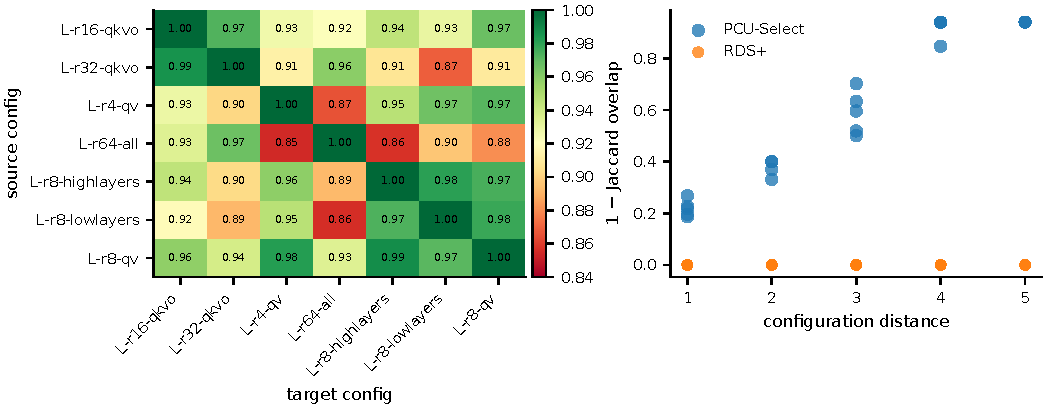
\includegraphics[width=\textwidth]{Figures/fig_config_sensitivity.pdf}
\caption{PCU-Select responds to configuration changes. \emph{Left:} Rows denote
the PEFT used for selection and columns the PEFT used for target training; each
column is normalized by its matched diagonal. The mean normalized off-diagonal
drop is $0.068$. On the unnormalized scale, the matched and mismatched means are
21.25 and 19.79, respectively, a $1.46$-point gap. \emph{Right:} Selection
difference, measured as $1-$Jaccard, versus the heuristic distance
$|\log_2 r_i-\log_2 r_j|+\mathbb{I}[\text{placement differs}]
+\mathbb{I}[\text{module set differs}]$. Across the 21 unordered pairs of seven
LoRA configurations, the descriptive Spearman correlation is $\rho=0.969$;
leave-one-configuration-out values span $[0.947,0.972]$. RDS+ lies at zero
because, for a fixed task, its ranking is PEFT-independent.}
\label{fig:config-sensitivity}
\end{figure*}

\paragraph{Unseen-configuration transfer.}
Table~\ref{tab:ood-levels} reports the values plotted in Figure~3 of the main paper.
Near-support targets transfer zero-shot.
Calibration closes most of the gap for far same-family targets and LN Tuning.
For Prefix/P-Tuning, the point estimate falls from 6.97 to 1.99 but leaves a
larger residual gap than for L1 or LN Tuning. The 0.18 change from Cal-200 to
Cal-500 is descriptive rather than evidence of a reliable difference between
the two label budgets.

\begin{table*}[t]
\centering
\small
\setlength{\tabcolsep}{4pt}
\begin{tabular}{lllrrr}
\toprule
Tier & Targets & Ref. & Zero-shot & Cal-200 & Cal-500 \\
\midrule
L0 & L-r32-qkvo, AD-b16 & LESS & 0.34$\pm$0.41 & -- & -- \\
L1 & L-r64-all, AD-b256, L-r8-highlayers & LESS & 2.08$\pm$0.44 & 0.91$\pm$0.29 & 0.30$\pm$0.36 \\
L2-BF & BF & LESS & 4.08$\pm$0.70 & 0.65$\pm$0.26 & 0.23$\pm$0.42 \\
L2-Prompt & PRE-l16, PT-l32 & RDS+ & 6.97$\pm$0.34 & -- & -- \\
\bottomrule
\end{tabular}
\caption{Performance drop from the named reference across GSM8K, HumanEval, and MMLU (reference minus PCU-Select; paired mean$\pm$sample SD over three target-training seeds). Lower is better; zero denotes parity. L0 uses zero-shot only. Calibration reduces far same-family and BitFit drops. Prefix/P-Tuning lack compatible labels.}
\label{tab:ood-levels}
\end{table*}


\subsection{Baseline Specifications}
\label{sec:appendix-baselines}

The three named baselines span two relevant axes: whether selection uses
gradients and whether its scoring signal depends on the target PEFT. They are
not single-factor ablations; the component ablations above isolate individual
PCU-Select design choices. We specify each implementation below so that the
comparison is auditable.

\paragraph{RDS+ (representation similarity).}
RDS+ operates on the 768-dimensional joint semantic embedding
$e_x^{\text{joint}}$ produced by the frozen sentence encoder. This is the
semantic component of PCU-Select's sample representation $z_x$. RDS+ neither
trains the encoder nor uses features learned by the PCU-Select scorer.

RDS+ first standardizes every pool embedding per feature. It forms the query by
averaging the 32 task-sketch embeddings and applies the same pool statistics. It
then $L_2$-normalizes the pool and query vectors and ranks candidates by cosine
similarity.

RDS+ is \emph{task-conditioned} through the sketch query but
\emph{PEFT-agnostic}: its ranking does not depend on the target configuration.
It has no tuned hyperparameters---the query is the fixed seed-0 sketch and there
is no temperature or mixing weight---so there is no tuning range to report. The
``+'' denotes the per-feature standardization applied before cosine, relative to
a plain embedding-nearest-neighbor selector.

\paragraph{Influence (shared-datastore gradient similarity).}
The Influence baseline builds one shared projected-gradient datastore from the
base model's intervention-site activations. It uses the JL projection and $L_2$
normalization specified in the reproducibility notes. Each candidate carries
signatures $g_x^\omega$ at the 24 sites. The task query $g_t^\omega$ pools and
renormalizes the sketch gradient at each site. Influence scores each candidate
with the plain cosine $\sum_{\omega}\cos(g_x^\omega, g_t^\omega)$ and applies
global top-$k$ without site weighting. Its PEFT-agnostic gradient source makes
the ranking independent of the target configuration. Influence therefore
provides a PEFT-agnostic shared-gradient reference; its comparison with
PCU-Select does not by itself isolate the effect of PEFT conditioning.

\paragraph{LESS (per-PEFT gradient influence).}
LESS is a per-configuration reimplementation of gradient-influence selection
following LESS~\cite{xia2024less}. It applies four steps to each target PEFT.
First, it warms up the target adapter for $200$ steps to obtain the optimization
state. Second, it extracts Adam-preconditioned gradients over the adapter's own
trainable parameters at each checkpoint. Third, it projects the gradients into a
target-specific low-dimensional datastore. Finally, it ranks candidates by their
projected-gradient influence on the 32-example task sketch and averages across
warmup checkpoints.

The first three steps build the datastore over the target adapter's own
trainable parameters. The datastore is therefore PEFT-specific but
task-independent. LESS constructs it once per PEFT and reuses it for every task
sketch. Only the final projected-gradient scoring step is task-specific.

It costs about $0.30$ GPU-hours per task, so $1.20$ covers all four task sketches
for one configuration. The per-target cost of a PEFT configuration is therefore
$62.0$ (datastore) $+\,1.20$ (four per-task rankings) $=63.2$ GPU-hours, already
spanning the full four-task evaluation; the five-PEFT registry cost is
$5\times63.2=316.0$. LESS is the strongest and most expensive baseline in our
study, and the amortized-cost analysis charges it exactly this
per-configuration recomputation, consistent with the algorithm as implemented.

\paragraph{Baseline configuration and tuning.}
Random has no hyperparameters. RDS+ uses the fixed representation-similarity
rule above with the shared $32$-example sketch as its only task input. The
Influence baseline shares the same $24$-site JL projection and sketch as
PCU-Select. We fix every baseline's hyperparameters before test-metric
evaluation.


% =========================================================
% Reproducibility Checklist
% =========================================================
% Check the AAAI-27 instructions to see whether this must be included
% in the main paper or submitted separately.
% If required inside the paper, uncomment the following line:
%
% \input{ReproducibilityChecklist.tex}

\end{document}
